\chapter[O Estudo de Caso]{O Estudo de Caso}

Neste capítulo será apresentado o estudo de caso desse trabalho. Na primeira seção será apresentado o contexto e a caracterização da organização do estudo de caso. Na segunda seção será apresentada a empresa contratada para o desenvolvimento do projeto. Na terceira seção será apresentada a caracterização do contrato e seu objeto, ou seja, a caracterização do projeto do qual os dados foram coletados. Na quarta seção será apresentada a solução aplicada na gestão do contrato e será analisada sua conformidade com o pensamento \textit{lean}, métodos ágeis e a legislação atual. E, finalmente, na quinta seção serão apresentadas a análise dos dados quantitativos e a discussão dos resultados.

\section[A Organização]{A Organização}

O organização escolhida, IPHAN, uma autarquia pública federal, possui uma força de trabalho atuante na área de TI de apenas 8 servidores, dos quais apenas 4 trabalham diretamente com sistemas. O perfil dessa equipe é apresentado na Tab. (\ref{piphan}). Devido ao número reduzido de servidores disponíveis na área de TI do órgão, frequentemente uma mesma pessoa acaba desempenhando diferentes papéis requeridos pela IN 04/2010.

\begin{table}[H]
\center
\footnotesize
\begin{tabular}{|c|c|c|}
\hline
\textbf{Área}          & \textbf{Perfil}   & \textbf{Quantidade} \\ \hline
TI Geral               & Coordenador de Tecnologia da Informação   & 1                   \\ \hline
Infraestrutura         & Analista de Tecnologia da Informação do MP   & 2                   \\ \hline
Sistemas               & Analista de Tecnologia da Informação do MP   & 2                   \\ \hline
\multirow{3}{*}{Apoio} & Analista de Tecnologia da Informação do MP   & 1                   \\ \cline{2-3} 
\multicolumn{1}{|l|}{} & Servidor do Ministério da Ciência, Tecnologia e Inovação & 1                   \\ \cline{2-3} 
\multicolumn{1}{|l|}{} & Servidor do IPHAN & 1                   \\ \hline
\end{tabular}
\caption{Perfil da Equipe do IPHAN}
\label{piphan}
\end{table}

O contexto atual do órgão foi identificado por meio da aplicação da técnica de entrevista informal, de questionário e da documentação disponível do órgão. O questionário aplicado pode ser encontrado no Apêndice A. Vale ressaltar que esse questionário foi aplicado não só para caracterização da organização como também para coleta de dados quantitativos necessários para o estudo de caso deste trabalho e ele foi projetado de forma generalizada para que tanto o IPHAN quanto a empresa contratada, EGL - Engenharia Ltda, pudessem respondê-lo.
 
Os fatores mais significantes que são gerenciados pela área de TI do órgão são:
\begin{itemize}
\item Atender as demandas para desenvolvimento de sistemas (sistema novo, manutenção, documentação).
\item Controlar a qualidade dos sistemas.
\item Possuir medições de sistemas.
\end{itemize}

Por meio do questionário foram identificados fatores que motivaram o uso de métodos ágeis na gestão do contrato do órgão.A Tab. (\ref{fm}) mostra a porcentagem dos fatores motivacionais citados pelos servidores da área de sistemas do órgão. 

\begin{table}[H]
\center
\footnotesize
\begin{tabular}{|c|c|}
\hline
\textbf{Fator Motivacional}          & \textbf{Porcentagem}  \\ \hline
Documentação desnecessária estava \\ sendo produzida e entregue               &  100\%                 \\ \hline
Entrega de \textit{software} funcional era pouco \\ frequente nos contratos anteriores        &  66\%                  \\ \hline
Visibilidade do processo era baixa              &  66\%                \\ \hline
O fiscal técnico do contrato e o gestor do \\ contrato não estavam exercendo os seus papéis como deveriam              &  66\%                \\ \hline
A qualidade do produto era preocupante   &  66\%                \\ \hline
Os requisitos de \textit{software} não eram atendidos &  66\%                \\ \hline
\end{tabular}
\caption{Fatores motivacionais}
\label{fm}
\end{table}

As metas norteadoras para a elaboração do processo de gestão de contrato com métodos ágeis foram:
\begin{itemize}
\item Ser aderente à legislação pertinente;
\item Entregar \textit{software} mais rapidamente;
\item Focar na gestão do contrato e na definição de uma metodologia de gestão de demandas;
\item Não focar em dizer como a empresa deveria desenvolver o \textit{software}, ou seja, não definir metodologia de desenvolvimento de \textit{software};
\item Satisfazer as necessidades do cliente.
\end{itemize}

Com isso, o IPHAN optou por definir uma metodologia ágil de gestão de contrato para o controle do órgão sobre as demandas e entregas de ordens de serviço. O IPHAN não definiu uma metodologia de desenvolvimento de \textit{software}, ou seja, o órgão não determina que a empresa siga uma metodologia ágil de desenvolvimento de \textit{software}, é necessário apenas que a empresa se adeque as restrições impostas independente de qual metodologia de desenvolvimento ela irá utilizar.

Outros instrumentos contratuais que foram modificados com a adoção do processo de gestão de contrato com métodos ágeis foram a forma de pagamento e a aplicação de multas. Em relação a esta, diferentemente das outras formas de gestão de contrato utilizadas anteriormente, onde as multas eram progressivamente aplicadas, por exemplo, sobre a não entrega de documentação, detinha caráter meramente punitivo. Com o novo processo, passou-se a considerar o maturidade e crescimento da empresa no contrato e  se não houvesse entrega de \textit{software}, a empresa contratada não recebia o pagamento estimado para aquela ordem de serviço. O faturamento das ordens de serviço era executado a cada entrega, final de \textit{sprint}, o que mantinha o fluxo de caixa da empresa contratada sempre ativo.


\section[A Empresa Contratada]{A Empresa Contratada}

A empresa contratada para desenvolvimento do projeto foi a empresa EGL - Engenharia Ltda. Formada por uma equipe multidisciplinar, a EGL Engenharia, desenvolve sistemas de informação geográfica e de apoio a gestão administrativa jurídica, privada ou pública. É capacitada a criar sistemas customizados para atender as necessidades especificas, além de fornecer manutenção corretiva e evolutiva destes.

A EGL - Engenharia Ltda possui entre 7 e 9 envolvidos no desenvolvimento do projeto.  O perfil dessa equipe é apresentado na Tab. (\ref{pegl}). É importante ressaltar que os perfis são apenas os papéis que cada integrante da equipe podia assumir, alguns integrantes eram mais especialistas em determinadas áreas que outro, no entanto, toda a equipe participou do processo de desenvolvimento do sistema. Portanto, a equipe não é uma equipe especialista, mais sim generalista, característica comum de equipes ágeis.

\begin{table}[H]
\center
\footnotesize
\begin{tabular}{|c|c|c|}
\hline
\textbf{Perfill}          & \textbf{Quantidade}  \\ \hline
Scrum Master               &  1                  \\ \hline
Desenvolvedor       &  2               \\ \hline
Analista de Requisitos              &   1                \\ \hline
Analista de Sistemas            &   1              \\ \hline
Arquiteto de Sistemas           &  1               \\ \hline
Analista de Georreferenciamento             &  1               \\ \hline
Preposto   &  1               \\ \hline
\end{tabular}
\caption{Perfil da Equipe da EGL - Engenharia Ltda}
\label{pegl}
\end{table}


No desenvolvimento do projeto a empresa utilizou a metodologia \textit{Scrum} e a linguagem de programação Java. No que diz respeito a experiência da equipe com essa metodologia, houve uma grande variação nas respostas do questionário, existindo cerca de 33\%  dos integrantes com pouca experiência, cerca de 33\% dos integrantes com experiência regular e cerca de 33\% integrantes com alta experiência. No que diz respeito a experiência da equipe com a liguagem de programação, 100\% dos desenvolvedores tinham uma alta experiência.

A lista de práticas ágeis utilizadas para o desenvolvimento do projeto são apresentadas na Tab. (\ref{praticasegl}).

\begin{table}[H]
\center
\footnotesize
\begin{tabular}{|c|c|c|}
\hline
Padrões de Codificação.              &   Revisão de Código.                \\ \hline
Refatoração de Código.     &  Testes de Fumaça (Smoke Testing), de Integração e de Aceitação.            \\ \hline
 Programação em Par.              &   Histórias de Usuário.               \\ \hline
Integração Contínua.         &   Planning Poker.             \\ \hline
Controle de Versão.          &   Planejamento das Iterações.               \\ \hline
Entregas Frequentes.            &   Backlog do Produto e da \textit{Sprint}.             \\ \hline
 Código Limpo.   &  Quadro Kanban.            \\ \hline
Burndown Charts.   &  Retrospectivas e Reunião Diária.        \\ \hline
Equipes Auto-organizadas.   &  Times Pequenos.           \\ \hline
\end{tabular}
\caption{Práticas Ágeis adotadas pela EGL - Engenharia Ltda}
\label{praticasegl}
\end{table}


\section[Caracterização do Projeto Contrato]{Caracterização do Projeto do Contrato}

\subsection[Visão Geral]{Visão Geral}

O IPHAN é responsável pela gestão de diversos processos de preservação do patrimônio cultural, como por exemplo, ações para sua identificação, proteção, gestão e fomento. Decorrente
de suas atribuições, o órgão produz uma grande quantidade de informações fragmentadas em termos territoriais e temáticos. Nos quatro anos anteriores ao contrato do SICG, o IPHAN elaborou uma metodologia
para definir os processos de cadastro, inventário e gestão do patrimônio cultural material. Essa metodologia tinha por objetivo geral abordar o Patrimônio Cultural de forma integrada, sistêmica
e estratégica, conforme detalhado a seguir:

\begin{itemize}
\item Integrada: cobrindo todas as categoriais do patrimônio material;
\item Sistêmica: estabelecendo moldes a serem utlizados nas diversas etapas de ações de preservação, possibilitando o "diálogo" e troca de informações entre áreas e etapas de trabalho;
\item Estratégica: considerando o mapeamento, a organização e a disponibilização de informações sobre o patrimônio como base para a construção de políticas públicas integradas - com outros parceiros - e de planos de preservação e desenvolvimento das regiões onde se inserem os bens.
\end{itemize}

Em termos específicos, a metodologia buscou, em primeiro lugar, mapear os procedimentos necessários para a execução das ações de cadastramento, proteção, normatização e fiscalização de bens culturais de natureza material, indicando adicionalmente os dados a serem coletados. Este mapeamento contou com a participação de representantes das Superintendências e Escritórios Técnicos, que, por meio de Grupos de Trabalho, analisaram, de forma crítica, as metodologias até então existentes.

A revisão dos processos levou à formulação da nova metodologia que, por sua vez, permitiu a otimização das atividades de cadastramento de sítios históricos e de bens tombados isoladamente e gerou a normalização das ações de fiscalização. O resultado desse trabalho produziu um conjunto de fichas e procedimentos específicos com demandas para cadastramento de dados textuais, geográficos e imagens.

Havia um entendimento no IPHAN de que era necessária a formação de uma rede de proteção fomentada pelo Sistema Nacional do Patrimônio Cultural (SNPC) que consolidasse o grande volume de informações atualmente produzido por suas unidades administrativas, composto de 27 Superintendências, 30 escritórios técnicos, 4 Unidades Especiais e 2 Parques Históricos Nacionais. Entretanto, a natureza das informações, em grande maioria armazenadas em planilhas e em banco de dados isolados, dificultava o processo de consolidação das informações. Esse fato frustava os esforços para a construção da rede de proteção baseada nos recursos e tecnologias atualmente adotados, pois demandava o aporte considerável de recursos financeiros e humanos sem ganhos no processo. O órgão se manteria refém da demora na produção de informações decorrente do intervalo entre ação e recepção das respostas, ou seja, entre a percepção do problema e sua solução.

Apesar do fato de os processos de cadastramento, normatização de sítios urbanos tombados e fiscalização de bens imóveis de metodologia já fazerem parte da realidade das Superintendências e Escritórios Técnicos, o processo manual de suporte e gestão dos dados tornava a execução precária e morosa.

A Tabela \ref{visao} apresenta a visão geral da situação vivida pela IPHAN, antes da solução informatizada, a qual subsidiava a contratação da solução informatizada.

\begin{table}[H]
\begin{tabular}{|l|l|}
\hline
\textbf{O que o IPHAN tinha?}                                                                                                                                                         & \textbf{O que o IPHAN não tinha?}                                                                                                     \\ \hline
\begin{tabular}[c]{@{}l@{}}Processos de Cadastramento, normatização,\\ tombamento e fiscalização revisados.\end{tabular}                                                              & Processos automatizados.                                                                                                              \\ \hline
\begin{tabular}[c]{@{}l@{}}Organização territorial sobre o contéudo\\ cultural (necessidade de vinculação entre\\ o bem cultural e o território e localização\\ física).\end{tabular} & \begin{tabular}[c]{@{}l@{}}Solução informatizada com\\ inteligência geográfica.\end{tabular}                                          \\ \hline
\begin{tabular}[c]{@{}l@{}}Cultura gerencial sobre os processos de\\ trabalho.\end{tabular}                                                                                           & \begin{tabular}[c]{@{}l@{}}Suporte informatizado para \\ tomada de decisão.\end{tabular}                                              \\ \hline
\begin{tabular}[c]{@{}l@{}}Grande volume de dados produzidos ao longo\\ dos últimos 3 anos de implantação da nova\\ metodologia.\end{tabular}                                         & \begin{tabular}[c]{@{}l@{}}Ferramentas adequadas para gestão\\ e disponibilização dos dados\\ existentes.\end{tabular}                \\ \hline
\begin{tabular}[c]{@{}l@{}}Grande volume de dados produzidos por outras\\ metodologias de cadastramento, normatização\\ de sítios urbanos e fiscalização.\end{tabular}                & \begin{tabular}[c]{@{}l@{}}Ferramentas e procedimentos\\ automatizados adequados para a\\ migração dos dados existentes.\end{tabular} \\ \hline
\end{tabular}
\caption{Visão geral da situação do IPHAN}
\label{visao}
\end{table}

Portanto, a solução informatizada era apontada como um caminho adequado para endereçar as dificuldades citadas, pois, possibilitaria a execução de vários processos do IPHAN (cadastramento, normatização, fiscalização e planejamento) de maneira integrada, garantindo agilidade na produção da informação. 

Com isso, o sistema que foi proposto, o SICG, foi formado por 7 módulos:

\begin{itemize}
\item Módulo 1 - Conhecimento;
\item Módulo 2 - Análise e Gestão;
\item Módulo 3 - Cadastro;
\item Módulo 4 -  Administração de Usuários;
\item Módulo 5 -  Fiscalização;
\item Módulo 6 - Cadastro Auxiliares;
\item Módulo 7 - Relatórios Adicionais.
\end{itemize}

\subsection[Objetivos da Contratação]{Objetivos da Contratação}

Os objetivos da contratação eram:

\begin{itemize}
\item Automatizar o processo de trabalho decorrente da metodologia de inventário, cadastramento, análise e gestão do patrimônio material, denominado Sistema Integrado de Conhecimento e Gestão (SICG);
\item Centralizar as diversas bases de informações utilizadas pelo Departamento de Patrimônio Material e Fiscalização (DEPAM) em uma base de dados única, possibilitando integração futura com bases de dados de outros departamentos do IPHAN,   o problema atual de falta de integração, da dispersão e da redundância dos dados;
\item Possibilitar a descontinuidade gradativa de 100\% das bases de dados isoladas, de caráter local ou descentralizado existentes no DEPAM;
\item Mapear as informações produzidas pelas diversas coordenações do DEPAM, pelas Superintendências e Escritórios Técnicos, pelos parceiros do Sistema Nacional de Patrimônio Cultural (SNPC), e as informações presentes no Arquivo Central do IPHAN, por meio de dados geográficos convergentes;
\item Possibilitar a realização de análises territoriais e de uma visão territorial das ações do DEPAM, provendo atributos de tamanho, proximidade, área, localização, topologia e outros, por meio de dados georreferenciados;
\item Consolidar informações originidas nas diversas coordenações do DEPAM, pelas Superintendências e Escritórios Técnicos, pelos parceiros do SNPC e uma base de dados geográfica de alta escalabilidade e que contenha 100\% das informações georreferenciadas;
\item Garantir celeridade no processo decisório, por meio da entrega de informações consistentes, precisos e que sejam entregues em tempo hábil, evitando ônus para a administração pública;
\item Possibilitar a redução do tempo e esforço necessário para a compilação das informações do DEPAM, advindas da recuperação e do cruzamento de produção das unidades do IPHAN de todo o pais. Espera-se que o tempo médio de resposta para compilação das informações seja reduzido de 30 dias para resposta em tempo real.
\end{itemize}


\subsection[Metodologia de Trabalho]{Metodologia de Trabalho}

\textbf{Forma de Encaminhamento das Ordens de Serviço}

Toda ordem de serviço era repassada pessoalmente ao preposto da contratada.

\textbf{Ciclos}

Todo o sistema foi desenvolvido de forma iterativa e incremental, por meio de ciclos, ao longo de toda a vigência contratual, até sua conclusão total. O desenvolvimento e, por consequência, o repasse de conhecimento à contratada será feito por ciclos de planejamento e reuniões de levantamento de requisitos e aprendizado. Cada ciclo tem duração de 2 a 4 semanas.

O Ciclo de Planejamento (\textit{Sprint} 0) tinha como objetivo o planejamento de todo o projeto.

Os Ciclo de Desenvolvimento (\textit{Sprints} de 1 a 24) tinha como objetivo o desenvolvimento do sistema.

O Ciclo de Implantação (Penúltima \textit{Sprint}) tinha como objetivo a implantação do sistema.

O Ciclo de Encerramento (Última \textit{Sprint}) tinha como objetivo o treinamento dos seus usuários e o encerramento do projeto.

\textbf{Reuniões}

Cada ciclo teve uma Reunião de Planejamento no início do mesmo e uma Reunião de Encerramento ao final do mesmo.

Na Reunião de Planejamento, a Contratada apresentou à Contratante uma proposta de Ordem de Serviço para o ciclo em planejamento. A Contratante emitiu parecer sobre a proposta. Aprovada a proposta, a Contratante, por meio de Ordem de Serviço, autorizou a Contratada a executar o ciclo planejado.

Na Reunião de Encerramento, a Contratada entregou e apresentou à Contratante o conjunto de produtos resultantes da execução do respectivo ciclo.

Os produtos entregues pela Contratada tinham um prazo de no máximo um ciclo para serem homologados pela Contratante.

\section[Caracterização da Solução]{Caracterização da Solução}

Para desenvolver uma metodologia de gestão de contratos \textit{software} baseada no Scrum e no Pensamento \textit{Lean}, o IPHAN definiu alguns procedimentos que deveriam ser feitos com o foco na minimização dos riscos da execução contratual e na obtenção do sucesso no contrato de terceirização. O \textit{framework} utilizado não foi considerado o mais relevante, mas sim os valores e princípios do Manifesto Ágil, além do atendimento à legislação vigente. 

As metodologias ágeis foram utilizadas como o meio para atingir o sucesso ou para identificar de forma rápida os riscos iminentes. O sucesso contratual pode ser entendido como aquele contrato que atende às necessidades do órgão, com sistemas, sem comprometer o erário (tesouro público). Assim, para atingir sucesso em um contrato é preciso que pelos menos esses três procedimentos sejam realizados: 
\begin{itemize}
\item Definir premissas nos artefatos desde o planejamento da contratação;
\item Alinhar diretrizes e condições com a Direção de TI;
\item Convalidar com a Alta Administração, ou seja, validar e sustentar essas diretrizes durante o contrato.
\end{itemize}

A lista de práticas ágeis utilizadas no projeto SICG para a gestão do contrato estão na Tab. (\ref{praticasiphan}).

\begin{table}[H]
\center
\footnotesize
\begin{tabular}{|c|c|c|}
\hline
 Definição de Pronto              &   Histórias de Usuário.              \\ \hline
Planejamento das Iterações.  &  Backlog do Produto.           \\ \hline
  Backlog da \textit{Sprint}.             &   Quadro Kanban.              \\ \hline
Burndown Charts.         &  Retrospectivas.            \\ \hline
Tempo de Ciclo (Lead time).         &  Revisão de Código.               \\ \hline
\end{tabular}
\caption{Práticas Ágeis adotadas pelo IPHAN}
\label{praticasiphan}
\end{table}


Com isso, foram definidas algumas premissas que orientaram o planejamento e execução do contrato. A saber: 
\begin{itemize}
\item O IPHAN não deveria definir, ou exigir, o uso de Metodologia Ágil da entidade contratada. Não defina Metodologia de Desenvolvimento de \textit{Software} (MDS), mas sim a
forma de gerenciar as demandas (ordens de serviço), os produtos que devem ser entregues e seus critérios de aceitação. 
\item A recontagem de Pontos por Função nos moldes do roteiro do SISP com metodologia ágil que pode mudar constantemente é um risco. É preciso alterar o percentual definido para a alteração, manutenção ou refatoração de uma funcionalidade, definir corretamente o conceito de manutenção evolutiva, refatoração e alteração de requisito e evidenciar no processo o custo de uma alteração e fazer com que o gestor negocial, que pediu a alteração, assine a ordem de serviço e ateste a nota fiscal;
\item Só abra uma Ordem de Serviço (OS) por vez e por projeto. Pode-se ter várias OS abertas com a mesma Contratada, porém, será uma OS para cada projeto e uma OS por \textit{Sprint}. Além disso, nunca comece oficialmente a próxima demanda sem receber ou finalizar a demanda anterior. Caso uma OS não estiver atendendo o que foi solicitado, ou por uma mudança negocial essa OS não for necessária, cancele-a e abra outra ordem de serviço que atenda a nova exigência do gestor contratual;
\item Não gerencie atrasos ou defeitos. No fim da \textit{Sprint}, receba o que estiver pronto, mesmo que não seja tudo que foi solicitado. Se nada foi entregue é uma ausência de entrega, não existe atraso, a \textit{Sprint} é considerada perdida. O produto não entregue ou com defeito dever voltar para fila de demandas e entrará na próxima OS ou \textit{Sprint} se o gestor negocial a quiser novamente, nunca aceite que corrijam um produto com defeito dentro da mesma OS;
\item Entenda a demanda antes de executá-la. É preciso planejar, pelo menos, com quantas ordens de serviço o projeto será validado, qual o processo de negócio que será desenvolvido, como será feita a gestão de demandas e qual será a demanda da próxima \textit{Sprint} ou OS;
\item Não aceite documentos sem sistemas. É importante ter em mente que não deve-se aceitar entregas apenas de documentação sem um produto funcional;
\item Acredite na evolução da empresa. No começo, a empresa contratada poderá não conseguir entregar o que foi solicitado ou entregar um produto funcional, no entanto, progressivamente ela irá se adequar ao processo e evoluir. 
\end{itemize} 

A partir dessas premissas definidas, a autarquia construiu um Kanban para auxiliar no processo de gestão de contratos.

O Kanban definido pelo IPHAN possui quatro colunas ou raias e está ilustrado na Fig. (\ref{kanban1})\footnote{Imagem disponível em http://www.slideshare.net/herbertparente/contratao-de-fbrica-de-software-metodologia-gil}.

\begin{figure}[H]
		\centering
		
			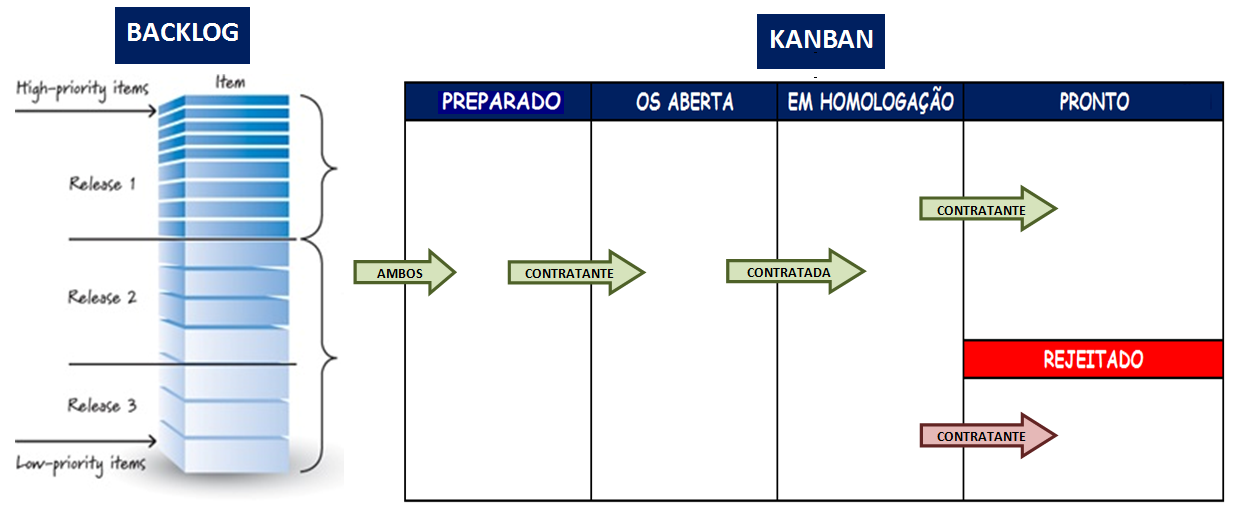
\includegraphics[scale=0.5]{figuras/kanbanIPHAN1.png}
		\caption{Quadro Kanban}
	\label{kanban1}
\end{figure}

A primeira raia do Kanban diz respeito aos itens que estão no estado “Preparado”. A condição de transição para esta raia pode ser feita da forma que o órgão quiser, Fig. (\ref{kanban2})\footnote{Imagem disponível em http://www.slideshare.net/herbertparente/contratao-de-fbrica-de-software-metodologia-gil}. Por exemplo, os itens com mais prioridade podem ser os primeiros a irem para esta coluna. É importante que a definição de “Preparado” e a definição de “Pronto” estejam bem claras para todos os envolvidos.  

\begin{figure}[H]
		\centering
		
			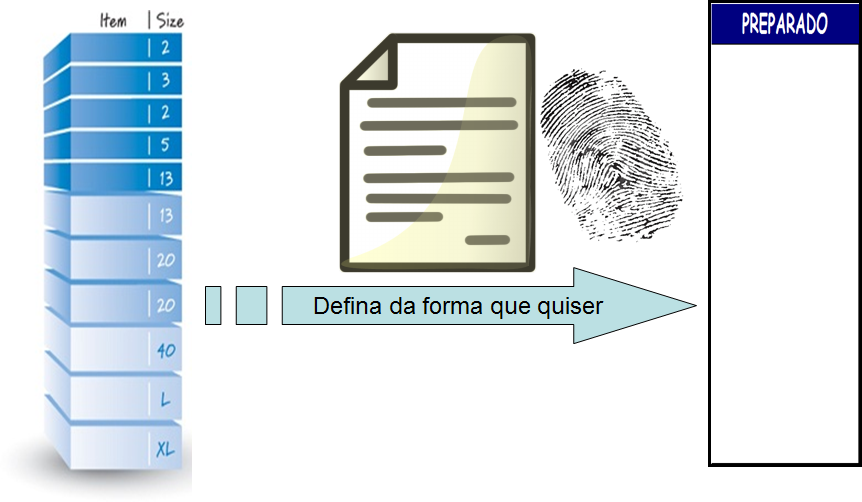
\includegraphics[scale=0.5]{figuras/kanbanIPHAN2.png}
		\caption{Transição para a raia Preparado}
		\label{kanban2}
\end{figure}

A transição de um item da raia “Preparado” para a raia “OS Aberta” ocorreu na abertura de uma ordem de serviço (Fig. (\ref{kanban3}))\footnote{Imagem disponível em http://www.slideshare.net/herbertparente/contratao-de-fbrica-de-software-metodologia-gil}. Esta transição ocorreu após o planejamento da \textit{sprint}, onde uma ordem de serviço de desenvolvimento era aberta com os itens que devem ser desenvolvidos para aquela \textit{sprint} e o desenvolvimento é iniciado. 

\begin{figure}[H]
		\centering
		
			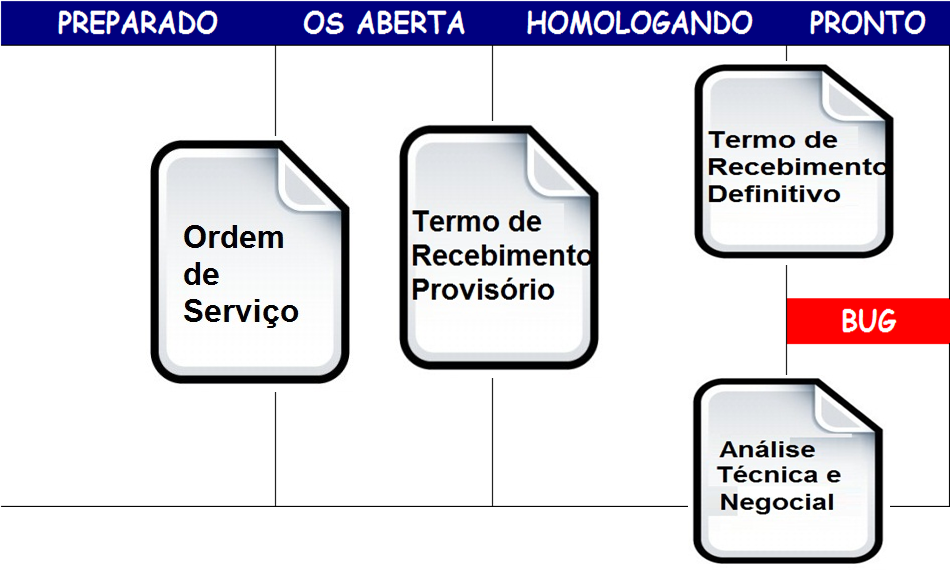
\includegraphics[scale=0.5]{figuras/kanbanIPHAN3.png}
		\caption{Transição entre raias}
		\label{kanban3}
\end{figure}

A transição da raia “OS Aberta” para a raia “Homologando” ocorreu quando o Termo de Recebimento Provisório era emitido (Fig. (\ref{kanban3})). Esta transição ocorreu ao se realizar o recebimento dos produtos e teve como saída o termo de recebimento provisório. Com a emissão do termo de recebimento provisório, os produtos recebidos entravam no processo de homologação. 

A transição da raia “Homologando” para a raia “Pronto” ocorreu quando o Termo de Recebimento Definitivo era emitido, ou seja, quando todos os produtos que foram anteriormente entregues eram verificados e aprovados (Fig. (\ref{kanban3})). Para tanto eram aferidos a aderência aos padrões técnicos e aos requisitos a partir de uma análise técnica e negocial, realizadas conjuntamente pelo Fiscal do Contrato e o Gestor do Contrato. Se fossen detectados defeitos nos produtos entregues ou se eles fossem rejeitados ou tivessem necessidade de refatoração, eles retornavam para a fila de demandas, iniciando novamente o ciclo. 

A sinalização de rejeitado ou \textit{bug} diz respeito a funcionalidade que foi rejeitada por não atender o que foi pedido tanto funcionalmente quanto tecnicamente. A sinalização de refatoração diz respeito a mudança que era pedida em uma funcionalidade depois de ela já ter sido implementada. Para que uma funcionalidade entre nessa sinalização era preciso que o gestor de negócio assumisse a responsabilidade pelos impactos que a mudança causará no custo, tempo e escopo.

Vale ressaltar que é importante que o trabalho em progresso (WIP) fosse limitado conforme o que é conceituado no método Kanban. O IPHAN definiu um limite de 210 Pontos por Função por ciclo de trabalho (Fig. (\ref{kanban4}) \footnote{Imagem disponível em http://www.slideshare.net/herbertparente/contratao-de-fbrica-de-software-metodologia-gil}). 

\begin{figure}[h]
		\centering
		
			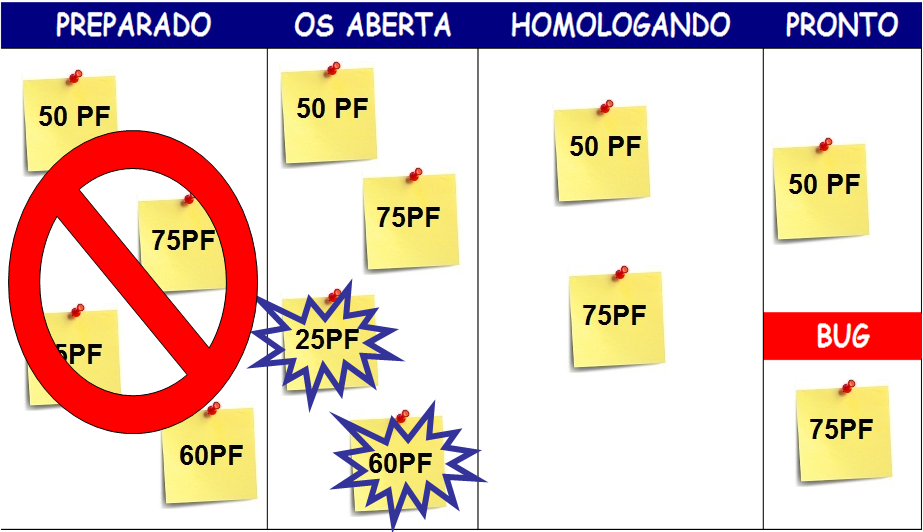
\includegraphics[scale=0.5]{figuras/kanbanIPHAN4.png}
		\caption{Limitação de WIP}
		\label{kanban4}
\end{figure}

É importante sempre valorizar a entrega de produto funcional e não pagar por apenas documentação. Assim, o IPHAN dividiu a forma de pagamento da contratada em percentuais, de acordo com a fase, valorizando a fase de execução, como ilustrado na Tab. (\ref{remuneracao}). Na \textit{Sprint} 18 do projeto SICG, ocorreu uma mudança acordada com a empresa contratada de modificar o pagamento da fase de execução para 100\%, porque não fazia sentido ter retenção de pagamento pois as fases de planejamento, desenvolvimento e encerramento já estavam sendo executadas pela empresa contratada, valorizando - se ainda mais a fase de execução.


\begin{table}[H]
\center
\footnotesize
\begin{tabular}{|p{6cm}|p{6cm}|}
  \hline
   \textbf{Fase} & \textbf{Percentual de Pagamento}\\
    \hline
   Planejamento (1 vez) & 5\%\\
   \hline    
   Execução (n vezes) & 75\%\\
    \hline
   Implantação (1 vez) & 10\%\\
   \hline
   Encerramento (1 vez) & 10\%\\
   \hline
\end{tabular}
\caption{Modelo de Remuneração do projeto SICG}
\label{remuneracao}
\end{table}


Outra técnica importante que foi construída diz respeito a parelização das atividades Fig. (\ref{kanban5})\footnote{Imagem disponível em http://www.slideshare.net/herbertparente/contratao-de-fbrica-de-software-metodologia-gil}. Enquanto uma ordem de serviço estava na etapa de homologação, outra ordem de serviço podia ser preparada, evitando que o fluxo do processo parasse e houvesse desperdício. 

\begin{figure}[H]
		\centering
		
			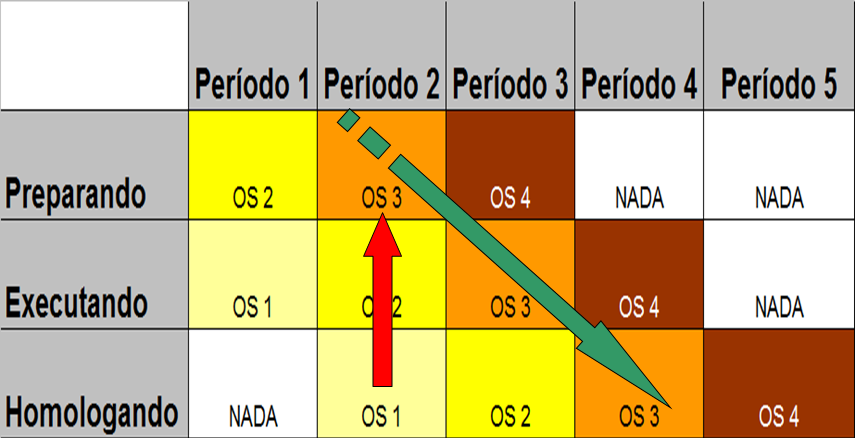
\includegraphics[scale=0.5]{figuras/kanbanIPHAN5.png}
		\caption{Parelização de Atividades}
		\label{kanban5}
\end{figure}

Após alguns meses de aplicação dessa solução o órgão deu início a construção da Metodologia IPHAN de Gestão de Demandas de Desenvolvimento Ágil de \textit{Software} (MIDAS). Uma parte do MIDAS, o mapeamento dos principais processos, pode ser visualizada no Anexo B.


\subsection[Análise da Adequação da Solução ao Pensamento Lean e ao Scrum]{Análise da Adequação da Solução ao Pensamento Lean e ao Scrum}

Ao analisarmos os princípios do Pesamento \textit{Lean}, apresentados no Capítulo 3, evidenciamos, na solução apresentada, a aplicação de alguns princípios de Desenvolvimento Lean, como: eliminação de desperdício, integração da qualidade, criação de conhecimento, entrega rápida, respeito as pessoas e a constância de propósitos. Ainda, identificamos as práticas gerenciamento de código, iterações curtas, participação do cliente e Kanban.

A parelização das atividades, Fig. (\ref{kanban5}), procurou reduzir alguns desperdícios de trabalho, ao evitar que o fluxo de trabalho fosse interrompido e, com isso, a produção, no que se refere ao desenvolvimento, fosse interrompida, à espera da finalização de uma determinada atividade. 

Considerando o ponto de vista do gestor do contrato e fiscal técnico, foi possível observar que a qualidade era integrada a cada ordem de serviço entregue por meio da aferição técnica. No entanto, essa aferição técnica realizada consistia em verificar se as classes estavam documentadas e se o modelo de dados era válido. Com relação a aferição técnica realizada pelo fiscal técnico, durante as \textit{sprints}, não evidenciamos a realização de utilização da prática de análise estática do código fonte. Esta técnica foi evidenciada apenas ao final do projeto por meio da contratação de uma outra empresa de qualidade, também terceirizada.

A criação do conhecimento pôde, por exemplo, ser evidenciada ao utilizar o aprendizado do processo definido nesta solução para a construção da metodologia de gestão de demandas do órgão, o MIDAS.

O IPHAN também definiu ciclos curtos de entrega de ordens de serviço, fazendo com que a entrega rápida de \textit{software} funcional acontecesse propiciando o \textit{feedback} constante do \textit{Product Owner} fosse possível. 

O respeito as pessoas pôde ser observado, por exemplo: i) ao considerar o aprendizado e adaptação da empresa contratada à solução de gestão de contratos definida; ii) a não aplicar multas punitivas; iii) a valorizar a fase de execução como principal fase de remuneração do trabalho. 

Observamos a constância de propósitos no que se refere a definição de objetivos claros da entrega de \textit{software} funcional.

O gerenciamento de código foi realizado por meio da ferramenta de controle de versão Apache Subversion (SVN). 

Foram definidas ciclos de produção curtos durante todo o projeto, as quais variaram de duas a quatro semanas.

A participação do cliente, desempenhada pelo \textit{Product Owner}, foi constante em todo o projeto. Ele sempre estava disponível para as dúvidas de requisitos.

As raias da ferramenta Kanban foram adaptadas para o contexto de contratações públicas e o trabalho em progresso foi limitado, o que corrobora com a teoria das restrições devido ao foco do IPHAN em controlar o fluxo de trabalho e não a metodologia de deesenvolvimento da contratada.

A limitação do trabalho em progresso realizada com a métrica Pontos por Função é resultado do conhecimento da capacidade produtividade da equipe. Neste trabalho não houve a investigação das limitações do Ponto por Função para medíção de tamanho e unidade de faturamento das ordens de serviço, uma vez que, este trabalho têm foco primário em ser exploratório.  

Não foram encontradas evidências, a partir dos dados coletados, da utilização dos princípios de adiar comprometimentos, de otimizar o todo, das práticas de teste automatizado e menos código. No que diz respeito a otimização do todo, não foi encontrada uma definição de cadeia de valor, onde a otimização seja feita desde a abertura da ordem de serviço até a implantação do \textit{software} junto ao usuário. Com relação ao teste automatizado, apesar da empresa contratada realizar alguns testes, não houve a entrega de uma base de código com uma suíte completa de testes automatizados. E com relação a prática menos código, segundo o IPHAN, foram encontradas muitas duplicações no código final do projeto, porém, essa métrica (código duplicado) não foi analisada nesse trabalho.

Ao analisarmos a metodologia Scrum, apresentada no Capítulo 4, identificamos que esta solução tem uma característica empírica e adaptativa conforme o Scrum. A utilização de iterações de curta duração e as cerimônias realizadas pelo IPHAN evidenciam a aderência a essa metodologia.

O IPHAN definiu cadências nas iterações ou \textit{sprints} com duração que variaram de duas a quatro semanas no máximo. O órgão juntamente com a empresa contratada realizou reuniões tanto de planejamento de cada \textit{sprint} quanto de restrospectiva de cada \textit{sprint} do projeto. 

O papel de \textit{Product Owner} foi desempenhado pelo gestor do contrato e o papel de Scrum Master pelo gestor de projeto da empresa contratada. Também foi utilizado o \textit{Product Backlog}, o qual continha todas as funcionalidades a serem desenvolvidas priorizadas. 

Não foram encontradas evidências, de acordo com os dados coletados, de que reuniões diárias e reuniões de revisão da \textit{sprint} eram realizadas. No que diz respeito a revisão da \textit{sprint}, ela era feita apenas pelo fiscal técnico no momento de homologação das funcionalidades entregues.

Em que pese não tenhamos medido especificamente a evidência de cada princípio, prática ou valor, pudemos observar indícios de que as premissas utilizadas como base para o desenvolvimento desta solução corroboram com a maioria dos princípios do Pensamento \textit{Lean} e com algumas práticas do \textit{Lean} no Desenvolvimento de \textit{Software} e da metodologia Scrum. No entanto, alguns princípios e práticas fundamentais não foram evidenciados, tais como otimização do todo, testes automatizados e menos código. 

Embora não tenhamos planejado no protocolo deste estudo caso a aferição de cada prática e princípio em particular, observamos ao longo deste estudo empírico o indício da aplicação destes. Como trata-se de um estudo exploratório, procuramos registrar o resultado dessas observações, de forma a balizar estudos posteriores.


\subsection[Análise da Adequação da Solução aos Valores Ágeis e a Legislação]{Análise da Adequação da Solução aos Valores Ágeis e a Legislação}

O projeto SICG, do contrato analisado neste estudo de caso, uma vez que é caracterizado como "serviço comum" foi contratado mediante a modalidade Pregão, na forma eletrônica, pelo critério de "menor preço", conforme os termos da Lei nº 8.666/93, apresentada no Capítulo 2.

É importante ressaltar que o Ácordão nº 237/2009 - Plenário do Tribunal de Contas da União orienta claramente sobre o uso da modalidade pregão para bens e serviços de tecnologia da informação considerados comuns e descarta que a complexidade, a criticidade ou a relevância dos bens possam justificar o não uso dessa modalidade.  E o Decreto nº 7.174/2010 Art. 9º, Parágrafo 1º declara a recomendação do tipo "menor preço" para a aquisição de bens e serviços de informática e automação considerados comuns. Com isso, no que diz respeito a modalidade e ao tipo da licitação, o IPHAN fez a definição adequada com respaldo da legislação pertinente. 

Conforme apresentado no Capítulo 2, a IN 04/2010 apresenta os papéis que estão presentes no processo de contratações e o mapeamento do processo da fase de Gerenciamento de Contrato. 

A Tabela \ref{rf} apresenta adequação de atores, papéis e responsabilidades do IPHAN aos papéis apresentados na IN 04/2010.

\begin{table}[H]
\center
\footnotesize
\begin{tabular}{|p{5.0cm}|p{4.0cm}|p{6.0cm}|}
\hline
\textbf{Atores IPHAN}                                                                                                                                                                                         & \textbf{Papéis IN 04/2010}                                                                  & \textbf{Responsabilidades}                                                                                                                                                                                                                                                                                                        \\ \hline
\begin{tabular}[c]{@{}l@{}}CGI– Coordenação de \\ Inventários e Conhecimento.\\ CGCI – Coordenação Geral \\ de Cidades.\\ DEPAM – Direção do \\ Departamento \\ de Patrimônio Material \\ e Fiscalização.\end{tabular} & \begin{tabular}[c]{@{}l@{}}Fiscal Requisitante\\ Gestor do Contrato\end{tabular} & \begin{tabular}[c]{@{}l@{}}- Gestão negocial do contrato.\\ - Aprovação do sistema.\\ - Auxílio no processo de definição de \\ regras do sistema.\\ - Solicitações de alterações.\\ - Repasse de informações sobre o \\ sistema.\\ - Homologação dos artefatos sistêmicos.\\ - Operação do sistema nas atividades \\ diárias.\end{tabular} \\ \hline
CGLOG – Coordenação Geral de Logística, Convênios e Contratos.                                                                                                                                          & Fiscal Administrativo                                                            & - Fiscalização administrativa do contrato.                                                                                                                                                                                                                                                                                        \\ \hline
CGTI – Coordenação Geral de Tecnologia da Informação.                                                                                                                                                   & \begin{tabular}[c]{@{}l@{}}Fiscal Técnico\\ Coordenador do \\ Projeto\end{tabular}  & \begin{tabular}[c]{@{}l@{}}- Fiscalização técnica do contrato.\\ - Coordenação técnica do projeto \\ quanto à solução, à documentação \\ sistêmica, à  metodologia \\ empregada e à arquitetura \\ tecnológica.\end{tabular}                                                                                                                 \\ \hline
Usuários nas Superintendências e outras unidades do IPHAN.                                                                                                                                              & Usuário                                                                          & \begin{tabular}[c]{@{}l@{}}- Auxílio no processo de definição de \\ regras e procedimentos existentes nas \\ Superintendências e outras unidades \\ do IPHAN.\\ - Operação do sistema nas atividades \\ diárias.\end{tabular}                                                                                                               \\ \hline
EGL - Engenharia                                                                                                                                                                                        & \begin{tabular}[c]{@{}l@{}}Preposto\\ Gestor do Projeto\end{tabular}             & \begin{tabular}[c]{@{}l@{}}- Acompanhar a execução do contrato.\\ - Atuar como interlocutor junto a \\ Contratante.\\ - Receber, diligenciar, encaminhar e \\ responder as principais questões \\técnicas, legais e administrativas \\ referentes ao andamento \\  contratual.\end{tabular}                                                  \\ \hline
\end{tabular}
\caption{Papéis e Responsabilidades}
\label{rf}
\end{table}

A Tabela \ref{gctiiphan} apresenta a análise da adequação da solução do IPHAN às etapas definidas na fase de Gerenciamento do Contrato da IN 04/2010, a qual é ilustrada na Fig. \ref{gcti}.

\begin{table}[H]
\center
\footnotesize
\begin{tabular}{|p{3.0cm}|p{4.0cm}|p{3.0cm}|p{4.0cm}|}
\hline
\multicolumn{2}{|c|}{\textbf{IN 04/2010}}                                                                                                                                                                               & \multicolumn{2}{c|}{\textbf{Solução IPHAN}}                                                                                                                        \\ \hline
\multicolumn{1}{|l|}{\textbf{Etapa}}                                                  & \textbf{Principais Atividades}                                                                                                  & \textbf{Fase}                    & \textbf{Principais Atividades}                                                                                                  \\ \hline
\multirow{4}{*}{Iniciação}                                                            & \begin{tabular}[c]{@{}l@{}}Elaborar Plano de\\ Inserção\end{tabular}                                                            & \multirow{4}{*}{Planejamento}    & \begin{tabular}[c]{@{}l@{}}Realizar Reunião\\ Inicial\end{tabular}                                                              \\ \cline{2-2} \cline{4-4} 
                                                                                      & \begin{tabular}[c]{@{}l@{}}Convocar Reunião\\ Inicial\end{tabular}                                                              &                                  & Planejar Projeto                                                                                                                \\ \cline{2-2} \cline{4-4} 
                                                                                      & \begin{tabular}[c]{@{}l@{}}Realizar Reunião \\ Inicial\end{tabular}                                                             &                                  & \begin{tabular}[c]{@{}l@{}}Realizar Ateste\\ Técnico\end{tabular}                                                               \\ \cline{2-2} \cline{4-4} 
                                                                                      & \begin{tabular}[c]{@{}l@{}}Enviar Ata para\\ Aprovação\end{tabular}                                                             &                                  & \begin{tabular}[c]{@{}l@{}}Realizar Aceitação da \\ Fase\end{tabular}                                                           \\ \hline
\multicolumn{2}{|c|}{Encaminhar Ordem de Serviço}                                                                                                                                                                       & Desenvolvimento                  & Planejar \textit{Sprint}                                                                                                                 \\ \hline
\multirow{9}{*}{\begin{tabular}[c]{@{}c@{}}Monitoramento \\ da Execução\end{tabular}} & Receber Objeto                                                                                                                  & \multirow{9}{*}{Desenvolvimento} & Acompanhar \textit{Sprint}                                                                                                               \\ \cline{2-2} \cline{4-4} 
                                                                                      & \begin{tabular}[c]{@{}l@{}}Elaborar Termo\\ de Recebimento\\ Provisório\end{tabular}                                            &                                  & \begin{tabular}[c]{@{}l@{}}Receber Produtos e \\ emitir Termo de \\ Recebimento Provisório\end{tabular}                         \\ \cline{2-2} \cline{4-4} 
                                                                                      & Avaliar Qualidade                                                                                                               &                                  & Realizar Ateste Técnico                                                                                                         \\ \cline{2-2} \cline{4-4} 
                                                                                      & \begin{tabular}[c]{@{}l@{}}Encaminhar Demandas\\ de Correção\end{tabular}                                                       &                                  & \begin{tabular}[c]{@{}l@{}}Elaborar Termo de \\ Recebimento Definitivo\\ das Funcionalidades\\ Homologadas\end{tabular}         \\ \cline{2-2} \cline{4-4} 
                                                                                      & \begin{tabular}[c]{@{}l@{}}Verificar Aderência\\ aos Termos Contratuais\end{tabular}                                            &                                  & \begin{tabular}[c]{@{}l@{}}Encaminhar Demandas \\ de Correção das \\ Funcionalidades Não \\ Homologadas\end{tabular}               \\ \cline{2-2} \cline{4-4} 
                                                                                      & \begin{tabular}[c]{@{}l@{}}Elaborar Termo de \\ Recebimento Definitivo\end{tabular}                                             &                                  & Emitir Nota Fiscal                                                                                                              \\ \cline{2-2} \cline{4-4} 
                                                                                      & \begin{tabular}[c]{@{}l@{}}Autorizar Emissão de\\ Nota Fiscal\end{tabular}                                                      &                                  & \begin{tabular}[c]{@{}l@{}}Verificar Regularidades \\ Fiscais, Trabalhistas e\\ Previdenciárias\end{tabular}                    \\ \cline{2-2} \cline{4-4} 
                                                                                      & \begin{tabular}[c]{@{}l@{}}Verificar Regularidades \\ Fiscais,Trabalhistas \\ e Previdenciárias\end{tabular}                    &                                  & \begin{tabular}[c]{@{}l@{}}Verificar manutenção \\ da necessidade,  \\economicidade \\ e oportunidade da \\ contratação.\end{tabular} \\ \cline{2-2} \cline{4-4} 
                                                                                      & \begin{tabular}[c]{@{}l@{}}Verificar manutenção \\ da necessidade, \\ economicidade \\ e oportunidade da \\ contratação.\end{tabular} &                                  & \begin{tabular}[c]{@{}l@{}}Realizar Aceitação\\ da Fase\end{tabular}                                                            \\ \hline
\multicolumn{2}{|c|}{Transição Contratual}                                                                                                                                                                              & \multicolumn{2}{c|}{Contratada deve passar documentos para transição}                                                                                                                          \\ \hline
\multicolumn{2}{|l|}{\multirow{3}{*}{Encerramento do Contrato}}                                                                                                                                                         & \multirow{3}{*}{Encerramento}    & Encerrar Projeto                                                                                                                \\ \cline{4-4} 
\multicolumn{2}{|l|}{}                                                                                                                                                                                                  &                                  & Realizar Ateste Técnico                                                                                                         \\ \cline{4-4} 
\multicolumn{2}{|l|}{}                                                                                                                                                                                                  &                                  & Realizar Aceitação da Fase                                                                                                      \\ \hline
\end{tabular}
\caption{Gerenciamento na IN 04/2010 x Gerenciamento no IPHAN}
\label{gctiiphan}
\end{table}


Conforme apresentado no Capítulo 4, o \citeonline{TCU:2013} identificou alguns riscos que poderiam comprometer a utilização de metodologias ágeis na gestão de contratos de fornecedores de desenvolvimento de \textit{software}. 

Assim como mencionamos na seção anterior, não planejamos formalmente a análise desses riscos, no protocolo deste estudo de caso. Portanto, não se trata de um estudo sitemático em investigar a materialização ou não dos riscos apontados por \citeonline{TCU:2013}, contidos na seção 4.3.1 do Capítulo 4. Contudo, registramos algumas observações, que foram possíveis de serem feitas com as fontes que analisamos. Não se trata, portanto, de um estudo aprofundado sobre esse fator, porém, reflete algumas percepções que emergiram no decorrer dessa investigação empírica. 

A Tab. (\ref{riscosiphan}) apresenta como o IPHAN lidou com cada um desses riscos.

\begin{longtable}{|p{2cm}|p{13cm}|}
\hline
\textbf{Riscos segundo Acórdão 2314/2013}                                                  & \textbf{Solução do IPHAN}                       \\ \hline
R1                                                                & A solução desenvolvida pelo IPHAN foi pensada para se adequar ao contexto de contratações de \textit{software}, com isso, algumas práticas e princípios ágeis não foram seguidos em sua plenitude. Porém os valores foram mantidos sem necessariamente desvirtuar da essência de ágeis. Não observamos, na documentação analisada, além do resultado das entrevistas e questionários, conflitos ou problemas de competência com a empresa contratada no que diz respeito a adaptação da metodologia de gestão de contratos definida. Vale ressaltar que a adaptabilidade é um dos pilares de qualquer método científico.          \\ \hline
R2                                                                &  As alterações realizadas na metodologia foram realizadas em comum acordo com a empresa contratada. Como exemplo, inicialmente a iteração de cada ordem de serviço tinha a duração máxima de três semanas, posteriormente, a duração máxima foi alterada para quatro semanas a pedido da empresa contratada em comum acordo com o órgão. É importante frisar nesse contexto, que o IPHAN não se preocupou em controlar e/ou definir uma metodologia de desenvolvimento para a empresa contratada. Preocupou-se em definir uma metodologia de gestão de contrato de desenvolvimento, focada no controle do fluxo de trabalho e no controle das restrições do sistema. Não se procurou em prescrever um método de gestão, materializado por um desenho de processos detalhados.               \\ \hline
R3                                                                & O IPHAN definiu no termo de referência os artefatos mínimos a serem entregues em cada fase do projeto. Na fase de Planejamento: plano de projeto e 3 propostas de identidade visual. Na fase de Desenvolvimento: plano de ciclo individual, código fonte (documentado), código compilado, modelo de entidade relacionamento, manual do sistema, manual do usuário e ajuda do sistema. Na fase de Implantação: manual do usuário e manual do sistema atualizados. Na fase de Encerramento: plano de treinamento, material de treinamento, relatório de encerramento do projeto com lições aprendidas e capacitação. Não identificamos alterações feitas sobre esse conjunto mínimo de artefatos.       \\ \hline
R4                                                                &  O IPHAN definiu no termo de referência os artefatos mínimos a serem entregues em cada fase do projeto. O pagamento a empresa durante a fase de desenvolvimento era realizado sobre as funcionalidades entregues e homologadas. Artefatos documentais, como o manual de usuário, eram exigidos durante a execução do projeto, porém foram apenas remunerados em sua versão final na fase de implantação ou encerramento. Observa-se o fato do IPHAN estar valorizando mais aspectos relacionados ao produto, do que preocupação demasiada com documentação exigida por um processo.             \\ \hline
R5                                                                & A definição de metodologia ágil de gestão de contrato foi definida pelo IPHAN já no instrumento convocatório.            \\ \hline
R6                                                                & O responsável pela área de negócios do IPHAN que desempenhou o papel de \textit{Product Owner} participou e colaborou constantemente com o desenvolvimento do projeto, exercendo também o papel de Gestor do Contrato. Algumas das atividades realizadas por ele foram: gerenciar funcionalidades, priorizar funcionalidades e realizar a homologação negocial dos artefatos entregues a cada iteração. \\ \hline
R7                                                                & O \textit{Product Owner} tinha pouco conhecimento sobre metodologias ágeis, assim como em fazer a priorização de funcionalidades essenciais para o bom desempenho do \textit{software}. Este risco materializou-se e foi tratado com a colaboração do fiscal técnico nas reuniões de planejamento da \textit{sprint}. Além disso, o \textit{Product Owner} se empenhou em aprender os aspectos técnicos e da metodologia.               \\ \hline
R8                                                                & No IPHAN, quando o \textit{Product Owner} afastou-se, em decorrência dos recessos de fim de ano, o desenvolvimento de novas funcionalidades foi suspenso e a empresa utilizou esse período para introduzir melhorias técnicas no produto, melhorando a qualidade do código e não paralisando o fluxo de trabalho do projeto. Isto ocorreu entre a \textit{sprint} 10 e 11. Quando o  \textit{Product Owner} afastou-se, na \textit{sprint} 16 em decorrência de férias, ele foi substituído por outro servidor do IPHAN da mesma área negocial sem ocorrer alteração no resultado da entrega.  \\ \hline
R9                                                                & De acordo com as respostas ao questionário aplicado, apesar do \textit{Scrum Master} da empresa contratada possuir pouca experiência em metodologias ágeis, os desenvolvedores possuiam uma experiência alta, de forma que não foi reportado pelo IPHAN problemas decorrentes desse risco, em que pese não analisamos esse fator de forma controlada. Uma sugestão seria que a empresa contratada fosse submetida a treinamentos para se adaptar mais rapidamente a metodologia ágil.              \\ \hline
R10                                                               &  Eram realizadas reuniões de planejamento e retrospectiva a cada ciclo com o \textit{Product Owner} e representantes da empresa contratada. Reuniões esporádicas também foram realizadas quando necessário, além de troca de e-mails, de forma que a comunicação entre contratante e contratada, foi observado pelos intrevistados como um fator positivo na relação.                \\ \hline
R11                                                               & A mudança de requisitos ocorreu  durante as \textit{sprints} do projeto. Com relação ao impacto sobre o custo do projeto, houve uma diferença de 1,8\% entre o custo planejado e o custo real ao final da \textit{sprint} 24. Com relação ao impacto sobre o prazo, foram planejados as mesmas quantidades de ciclos de desenvolvimento que foram realizados (24 ciclos), sendo que cerca de 78\% dos requisitos foram atendidos ao final da \textit{sprint} 24.         \\ \hline
R12                                                               & A paralelização de atividades ocorreu no IPHAN. Enquanto um ciclo entregue era homologado outro iniciava-se e era desenvolvido. Caso houvesse funcionalidades não homologadas no ciclo anterior, as mesmas eram passadas para o próximo ciclo. Não encontramos evidência de que esta prática tenha ocasionado diretamente atrasos na entrega do produto.             \\ \hline
R13                                                               & No IPHAN, o planejamento foi iniciado de forma global por meio da elaboração de um cronograma do projeto e, posteriormente, de forma mais específica nas reuniões de planejamento da \textit{sprint}. Não realizamos um estudo específico para analisar esse efeito sobre o custo total do projeto.             \\ \hline
R14                                                               & O valor pago no final de cada ciclo era realizado apenas sobre as funcionalidades que foram homologadas. Com relação a mudanças realizadas sobre funcionalidades já homologadas o IPHAN pagava 50\% do valor do ponto de função. Este percentual foi alterado com relação ao percentual constante no roteiro do SISP para minimizar o custo desse risco.           \\ \hline
R15                                                               & O IPHAN disponibilizou de forma tardia o \textit{software} desenvolvido em ambiente de produção, apenas ao final do projeto, contradizendo um dos objetivos dos métodos ágeis que é entrega adiantada e contínua de \textit{software} funcional "nas mãos" dos usuários. Isto causou a detecção tardia de erros. Porém, como havia uma garantia de cerca de doze meses após a finalização do contrato, os erros identificados foram corrigidos pela empresa contratada sem um novo pagamento ser necessário. Não avaliamos os impactos na percepção de uso, por parte dos usuários.            \\ \hline
R16                                                               &  Para mitigar esse risco, o IPHAN valorizou a fase de execução mais do que as outras, fazendo com que ela correspondesse a 75\% da remuneração total do projeto. Além disso, o IPHAN deixou aberto para a empresa contratada a possibilidade de utilizar outra métrica desde que a empresa apresentasse uma referência bibliográfica adequada e uma justificativa formal para o uso da mesma.              \\ \hline

\caption{Riscos Acórdão 2314/2013 x Solução IPHAN}
		\label{riscosiphan}
\end{longtable}

Ainda, como apresentado no Capítulo 4, o Acórdão nº 2314/2013 apresentou uma análise subjetiva com relação ao uso dos valores ágeis em contratações, relacionada a possibilidade de ferir os princípios da APF. A Tab. (\ref{apfiphan}) apresenta como o IPHAN lidou com os princípios da APF juntamente com os valores ágeis.

\begin{table}[H]
\center
\footnotesize
\begin{tabular}{|p{6cm}|p{8cm}|}
  \hline
   \textbf{Valor do Manifesto Ágil e Princípio da APF} & \textbf{Solução IPHAN}\\
    \hline
  Indivíduos e interações acima de processos e ferramentas e Princípio da Eficiência e Princípio de Pessoalidade &  Os processos da organização não foram desprezados. Segundo relatos dos entrevistados, quando uma solicitação da área requisitante era recebida, procurava-se verificar se eles tinham o processo de negócio daquela requisição mapeado. Caso não tivesse, era recomendado, porém não obrigatório, um mapeamento desses processos antes da demanda passar para o desenvolvimento.  Como forma de mitigar a relação de pessoalidade entre os funcionários da contratada e os gestores da instituição contratante, as reuniões de planejamento e restrospectiva foram todas registradas em ata de reunião. \\
   \hline    
 \textit{Software} operante acima de documentações grandes e completas e Princípio da Eficiência & Conforme o valor apresentado, o IPHAN valorizou a entrega de \textit{software} funcional acima de documentação abrangente. Ainda sim, houve uma preocupação de se valorizar a documentação do \textit{software} desenvolvido. Isso pode ser observado em nível de documentação de código, onde foi exigida a documentação por classe, método, arquivo, pacote e entre outros, em aderência a premissa de melhoria da manutenibilidade. Além disso, um conjunto
mínimo de artefatos foi exigido no instrumento
convocatório. Vale ressaltar que segundo o IPHAN, um documento que poderia ter sido acrescentado era o documento de regras de negócio.\\
    \hline
  Colaboração do cliente acima de negociações contratuais e Princípio da Vinculação ao Instrumento Convocatório &  O instrumento convocatório determinou qual era o processo de gestão de contratos do órgão assim como as alterações previstas. O \textit{Product Owner} do IPHAN estava frequentemente à disposição da equipe da empresa contratada para solucionar dúvidas com relação aos requisitos.\\
   \hline
  Responder à mudanças acima de seguir um plano e Princípio do Planejamento e Princípio da Economicidade & Um planejamento global foi realizado no inicío do contrato e planejamentos específicos realizados a cada ciclo. No momento em que um ciclo (com duração de quatro semanas) era planejado ele não poderia ser alterado, as alterações ficavam para uma iteração posterior, não ferindo o princípio do planejamento. Além disso, as iterações curtas adotadas pelo IPHAN facilitaram as mudanças. As mudanças realizadas por motivos técnicos não eram pagas novamente, não ferindo o princípio de economicidade. No entanto, as mudanças negociais eram tratadas com mais rigor, o \textit{Product Owner} assumia a responsabilidade sobre o impacto no custo, no tempo e no escopo. Essas mudanças de funcionalidades já homologadas eram remuneradas com 50\% do valor do ponto de função. \\
   \hline
\end{tabular}
\caption{Valores do Manifesto Ágil e Princípios da APF x Solução do IPHAN}
\label{apfiphan}
\end{table}

Ressaltamos novamente que não se trata de estudo exaustimos sobre os efeitos observados no riscos apontados em \citeonline{TCU:2013}, o que ensajaria estudos mais controlados para dimunir os viézes da observação.


\section[Análise dos Dados]{Análise dos Dados}

Nesta seção serão apresentados os resultados dos dados coletados, categorizados em três efeitos: entrega de ordens de serviço, satisfação do cliente e qualidade interna do código fonte. É importante destacar que é a partir da análise desses efeitos que responderemos às questões específicas elaboradas para investigar o problema apresentado. As subseções a seguir têm o objetivo de responder diretamente às questões específicas definidas no Capítulo 5.

\subsection[Efeitos sobre a entrega de ordens de serviço]{Efeitos sobre a entrega de ordens de serviço}

A partir dos dados coletados da documentação dos Processos do projeto SICG foram calculadas as métricas para responder as questões específicas QE1 a QE9, que caracterizam os efeitos sobre a entrega de ordens de serviço do uso de métodos ágeis na gestão do contrato de fornecedores de desenvolvimento de \textit{software}.

A Tabela \ref{resultadosmetricas} apresenta os resultados das métricas para cada uma das questões específicas anteriormente mencionadas.

\begin{table}[h]
\begin{tabular}{|p{2.0cm}|p{9.0cm}|p{5.0cm}|}
\hline
\textbf{ID} & \textbf{Questão}                                                                                                                                  & \textbf{Resultado da Métrica}    \\ \hline
QE1.        & Qual a quantidade total de ordens de serviço?                                                                                                    & 25 ordens de serviço          \\ \hline
QE2.        & Qual a quantidade de ordens de serviço que tiveram entrega de \textit{software} funcional?                                                                & 20 ordens de serviço          \\ \hline
QE3.        & Qual a quantidade de ordens de serviço que tiveram entrega apenas de documentação?                                                               & 1 ordem de serviço            \\ \hline
QE4.        & Qual a proporção de entrega de \textit{software} funcional?                                                                                               & 80\%                          \\ \hline
QE5.        & Qual a duração média de entrega de \textit{software} funcional?                                                                                           & 3.7 semanas                   \\ \hline
QE6.        & Qual a quantidade de ordens de serviço que não teve entrega de \textit{software} funcional e  de documentação?   & 4 ordens de serviço           \\ \hline
QE7.        & Qual a porcentagem de requisitos atendidos em cada ordem de serviço?                                                                             &  Tabela \ref{porcentagemrequisitos} \\ \hline
QE8.        & Quantas multas foram aplicadas no contrato?                                                                                                      & 0 multas                      \\ \hline
QE9.        & Qual o custo de cada \textit{sprint} e ordem de serviço do projeto?                                                                                       & Tabela \ref{custo}                 \\ \hline
\end{tabular}
\caption{Resultados Métrica de QE1. a QE9.}
		\label{resultadosmetricas}
\end{table}


A Tabela \ref{porcentagemrequisitos} apresenta a porcentagem de requisitos atendidos em cada ordem de serviço ou \textit{sprint}, respondendo assim a questão específica QE7.

\begin{table}[H]
\center
\begin{tabular}{|l|l|l|}
\hline
\textbf{\textit{Sprint}} & \textbf{OS} & \textbf{\begin{tabular}[c]{@{}l@{}}Porcentagem de\\   Requisitos Atendidos\end{tabular}} \\ \hline
0               & 1           & 100\%                                                                                    \\ \hline
1               & 2           & 0\%                                                                                      \\ \hline
2               & 3           & 94\%                                                                                     \\ \hline
3               & 4           & 0\%                                                                                      \\ \hline
4               & 5           & 94\%                                                                                     \\ \hline
5               & 6           & 100\%                                                                                    \\ \hline
6               & 6.1         & 0\%                                                                                      \\ \hline
7               & 7           & 100\%                                                                                    \\ \hline
8               & 8           & 94\%                                                                                     \\ \hline
9               & 9           & 100\%                                                                                    \\ \hline
10              & 10          & 100\%                                                                                    \\ \hline
11              & 11          & 100\%                                                                                    \\ \hline
12              & 12          & 100\%                                                                                    \\ \hline
13              & 13          & 84\%                                                                                     \\ \hline
14              & 14          & 100\%                                                                                    \\ \hline
15              & 15          & 100\%                                                                                    \\ \hline
16              & 16          & 100\%                                                                                    \\ \hline
17              & 17          & 84\%                                                                                     \\ \hline
18              & 18          & 0\%                                                                                      \\ \hline
19              & 19          & 100\%                                                                                    \\ \hline
20              & 20          & 100\%                                                                                    \\ \hline
21              & 21          & 100\%                                                                                    \\ \hline
22              & 22          & 36\%                                                                                     \\ \hline
23              & 23          & 60\%                                                                                     \\ \hline
24              & 24          & 100\%                                                                                    \\ \hline
\end{tabular}
\caption{Porcentagem de Requisitos Atendidos por Ordem de Serviço}
		\label{porcentagemrequisitos}
\end{table}

 A média geral de requisitos atendidos ao longo do projeto de acordo com os dados levantados da documentação foi de 78\%, o que coincide com a percepção dos envolvidos no projeto: 75\% dos envolvidos responderam ao questionário que a percepção geral de requisitos atendidos durante o projeto estava entre 70\% e 90\%.

A Tabela \ref{custo} apresenta o custo de cada ordem de serviço ou \textit{sprint}, respondendo assim a questão específica QE9. Como pode ser observado, nas ordens de serviço que tiverem a porcentagem de requisitos atendidos como 0\% não houve remuneração para a contratada. O custo estimado do contrato antes da contratação era de R\$ 990,000. Portanto, o custo final foi próximo do custo estimado, ultrapassando apenas 1,8\%.


\begin{table}[H]
\center
\begin{tabular}{|l|l|l|}
\hline
\textbf{Sprint}                                                  & \textbf{OS} & \textbf{Custo}                        \\ \hline
\begin{tabular}[c]{@{}l@{}}Planejamento\\   Inicial\end{tabular} & 1           & R\$                    49,500.00      \\ \hline
1                                                                & 2           & R\$                                 0.00 \\ \hline
2                                                                & 3           & R\$                    53,316.25      \\ \hline
3                                                                & 4           & R\$                                 0.00 \\ \hline
4                                                                & 5           & R\$                    36,382.50      \\ \hline
5                                                                & 6           & R\$                    31,927.50      \\ \hline
6                                                                & 6.1         & R\$                                 0.00 \\ \hline
7                                                                & 7           & R\$                    45,478.13      \\ \hline
8                                                                & 8           & R\$                    31,741.88      \\ \hline
9                                                                & 9           & R\$                    29,143.13      \\ \hline
10                                                               & 10          & R\$                    65,896.88      \\ \hline
11                                                               & 11          & R\$                    64,597.50      \\ \hline
12                                                               & 12          & R\$                  107,291.25       \\ \hline
13                                                               & 13          & R\$                    56,801.25      \\ \hline
14                                                               & 14          & R\$                    39,909.38      \\ \hline
15                                                               & 15          & R\$                    63,669.38      \\ \hline
16                                                               & 16          & R\$                    61,627.50      \\ \hline
17                                                               & 17          & R\$                    31,185.00      \\ \hline
18                                                               & 18          & R\$                                 0.00 \\ \hline
19                                                               & 19          & R\$                    53,831.25      \\ \hline
20                                                               & 20          & R\$                    50,490.00      \\ \hline
21                                                               & 21          & R\$                    63,112.50      \\ \hline
22                                                               & 22          & R\$                    13,612.50      \\ \hline
23                                                               & 23          & R\$                    22,027.50      \\ \hline
24                                                               & 24          & R\$                    36,630.00      \\ \hline
\end{tabular}
\caption{Custo por Ordem de Serviço}
		\label{custo}
\end{table}



É importante destacar que apesar das \textit{sprints} 1, 3, 6 e 18 não tiverem sido faturadas, não houve aplicação de multa para a contratada. Pois, conforme a solução caracterizada anteriormente, o órgão optou por modificar o modelo de remuneração e considera o aprendizado e a adaptação da empresa ao tipo de metodologia de gestão de contrato que está sendo aplicado. Além disso, o fato de a empresa não ter um pagamento em seu fluxo de caixa já é penalização suficiente para que a empresa faça a adequação do seu processo de trabalho.

Outro fato importante é que ao entregar uma ordem de serviço para homologação, uma recontagem de pontos por funções do que foi entregue era realizada, e ao realizar a homologação o fiscal técnico do IPHAN realizava uma nova contagem de pontos por função sobre as funcionalidades homologadas. Apenas o valor de pontos de função das funcionalidades homologadas eram faturados. Cada ponto de função corresponde a R\$ 495,00. Até a \textit{Sprint} 17 era realizado o pagamento de 75\% do valor homologado, no entanto, a partir da \textit{Sprint} 18, o valor do pagamento realizado passou a ser 100\% do valor homologado.

Ainda, pelos dados coletados neste estudo, não foi evidenciada a utilização de uma técnica de gerenciamento de custos do projeto, como exemplo, o valor agregado. Uma ferramenta que automatize o processo de acompanhamento de custos poderia prover uma informação mais adequada e poderia auxiliar o gestor na tomada de decisão. O gestor do contrato poderia analisar, por exemplo, se o que está sendo pago está de acordo com o que está sendo produzido ou de acordo com o que foi planejado.

\subsection[Efeitos sobre a satisfação do cliente]{Efeitos sobre a satisfação do cliente}

O cliente do projeto SICG é representado pelo papel de \textit{Product Owner}, que também atuou como gestor do contrato, e por todos os envolvidos no projeto por parte do IPHAN. Este nunca havia participado anteriormente de um projeto onde a gestão do contrato era realizada com o uso de métodos ágeis, portanto, a experiência dos envolvidos no projeto com esses métodos era pouca. Para coletar a opinião do cliente acerca das questões específicas QE10  e QE11 foi aplicado o questionário encontrado no Apêndice A.

A Figura \ref{visibilidade} apresenta a visibilidade do processo de todos os envolvidos no projeto por parte do IPHAN. Cerca de 80\% dos envolvidos no projeto considerou a visibilidade do processo como "Alta", dentre eles o gestor do contrato.

\begin{figure}[H]
		\centering
			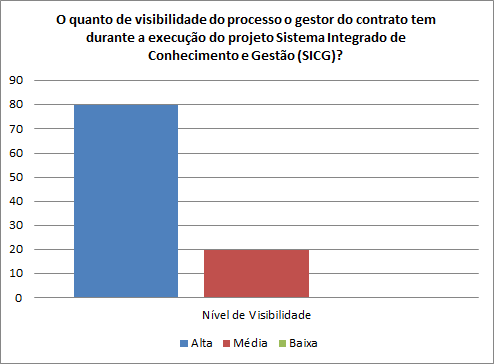
\includegraphics[scale=1.0]{figuras/visibilidade.png}
		\caption{Nível de Visibilidade do Processo do Projeto SICG}
		\label{visibilidade}
\end{figure}

A Figura \ref{satisfacao} apresenta o resultado de satisfação do IPHAN com relação ao produto entregue. De forma unânime foi considerado como "Satisfeito" o produto entregue pela empresa contratada. 

\begin{figure}[H]
		\centering
			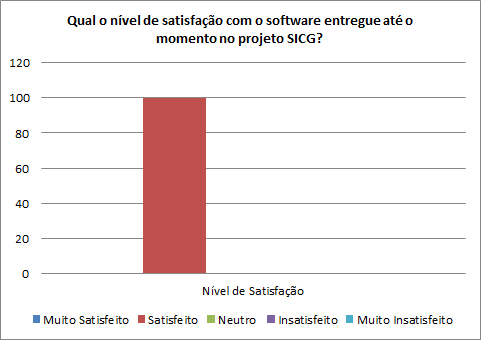
\includegraphics[scale=1.0]{figuras/satisfacao.png}
		\caption{Nível de Satisfação do Produto Entregue do Projeto SICG}
		\label{satisfacao}
\end{figure}

\subsection[Efeitos sobre a qualidade do código]{Efeitos sobre a qualidade do código}

A qualidade do código fonte do SICG pode ser avaliada por meio de métricas que evidenciam a qualidade externa \cite{ISO25023}. Neste trabalho foram selecionadas doze métricas de código fonte levantadas e categorizadas por \citeonline{Meirelles2013}: métricas de tamanho e complexidade e métricas de orientação à objetos. A definição dessas métricas pode ser encontrada no Apêndice B.


Um dos objetivos científicos do estudo de \citeonline{Meirelles2013} foi a identificação das distribuições estatísticas dos valores das métricas apresentadas anteriormente em 38 projetos de \textit{software} livre, onde foram analisadas 344.872 classes das aplicações mais utlizadas de \textit{software} livre, tais como, Chrome, Firefox, OpenJDK e VLC. A partir de cada uma das distribuições estatísticas \citeonline{Meirelles2013} classificou as métricas de código fonte de acordo com a frequência dos valores apresentados,
com os intervalos: muito frequente, frequente, pouco frequente e não frequente. Para simplificar o entendimento das métricas de código fonte, Morais interpretou os rótulos dos
intervalos de frequência definidos por \citeonline{Meirelles2013} em em rótulos qualitativos, tal como apresentado na Tab. (\ref{nomes}). 

\begin{table}[!ht]
	\begin{center}
	 \begin{tabular}{|l|l|}
		\hline
		\textbf{Intervalo de Frequência} & \textbf{Rótulo Qualitativos} \\ \hline
		Muito Frequente & Excelente \\ \hline
		Frequente       & Bom       \\ \hline
		Pouco Frequente & Regular   \\ \hline
		Não Frequente   & Ruim      \\ \hline
		\end{tabular}
		\caption{Nome dos Intervalos de Frequência e Qualitativos}
		\label{nomes}
		\end{center}
		\end{table}


Posteriormente, é apresentando na Tab. (\ref{intervalos}), retirada do
estudo de \citeonline{Meirelles2013}, com os intervalos encontrados para C++ e Java. Com isso, os intervalos apresentados na Tab. (\ref{intervalos}) foram os utilizados como os indicadores
de qualidade de código fonte na análise deste estudo de caso. É importante ressaltar que quando apresentarmos o resultado da análise sobre o código fonte deste estudo de caso e dissermos que o código fonte tem um rótulo "Excelente" ou "Ruim" para determinada métrica, siginifica dizer que, esse código fonte é "Excelente" ou "Ruim" em comparação ao melhor projeto de \textit{software} livre selecionado por \citeonline{Meirelles2013} na Linguagem Java, que foi o Open JDK8.


	
\begin{longtable}{|l|l|l|}
		\hline
		
		\textbf{Métrica} & \textbf{Rótulos Qualitativos} &  \textbf{Intervalos Qualitativos}  \\ \hline
		 % Métrica de Tamanho e Complexidade


		 %------------------------------- Tomcat
		 \multirow{4}{*}{LOC} 
		 & Excelente & [de 0 a 33]  \\
		 & Bom & [de 34 a 87]] \\
		 & Regular & [de 88 a 200]  \\
		 & Ruim & [acima de 200] \\ \hline
		 %---------------------------------

		 %-------------------------------  Tomcat	
		 \multirow{4}{*}{ACCM} 
		 & Excelente & [de 0 a 2,8]  \\
		 & Bom & [de 2,9 a 4,4]  \\
		 & Regular & [de 4,5 a 6,0]  \\
		 & Ruim & [acima de 6]  \\ \hline
		 %---------------------------------


		 %--------------------------------- Tomcat
		 \multirow{4}{*}{AMLOC} 
		 & Excelente & [de 0 a 8,3]  \\
		 & Bom & [de 8,4 a 18]  \\
		 & Regular & [de 19 a 34]  \\
		 & Ruim & [acima de 34]  \\ \hline
		 %---------------------------------

		 % Métricas de Orientação à Objetos

		 %------------------------------- Tomcat
		 \multirow{4}{*}{ACC} 
		 & Excelente & [de 0 a 1] \\
		 & Bom & [de 1,1 a 5]  \\
		 & Regular & [de 5,1 a 12] \\
		 & Ruim & [acima de 12] ] \\ \hline
		 %---------------------------------


		 %--------------------------------- Tomcat
		 \multirow{4}{*}{ANPM} 
		 & Excelente & [de 0 a 1,5] \\
		 & Bom & [de 1,6 a 2,3] ] \\
		 & Regular & [de 2,4 a 3,0]  \\
		 & Ruim & [acima de 3] \\ \hline
		 %---------------------------------

		 %--------------------------------- Tomcat
		 \multirow{4}{*}{CBO} 
		 & Excelente & [de 0 a 3]  \\
		 & Bom & [de 4 a 6] ] \\
		 & Regular & [de 7 a 9]  \\
		 & Ruim & [acima de 9] \\ \hline
		 %---------------------------------

		 %------------------------------- Tomcat
		 \multirow{4}{*}{DIT} 
		 & Excelente & [de 0 a 2]   \\
		 & Bom & [de 3 a 4]  ] \\
		 & Regular & [de 5 a 6]   \\
		 & Ruim & [acima de 6]  \\ \hline
		 %---------------------------------

		 %------------------------------- Tomcat
		 \multirow{4}{*}{LCOM4} 
		 & Excelente & [de 0 a 3]  \\
		 & Bom & [de 4 a 7]  \\
		 & Regular & [de 8 a 12]   \\
		 & Ruim & [acima de 12]  ] \\ \hline
		 %---------------------------------



		 %------------------------------- Tomcat
		 \multirow{4}{*}{NOC} 
		 & Excelente & [0]  \\
		 & Bom & [1 a 2]   \\
		 & Regular & [3]  ] \\
		 & Ruim & [acima de 3]   \\ \hline
		 %---------------------------------



		 %------------------------------- Tomcat 
		 \multirow{4}{*}{NOM} 
		 & Excelente & [de 0 a 8]   \\
		 & Bom & [de 9 a 17]   \\
		 & Regular & [de 18 a 27]  \\
		 & Ruim & [acima de 27]   \\ \hline
		 %---------------------------------




		 %--------------------------------- Tomcat
		 \multirow{4}{*}{NPA} 
		 & Excelente & [0]   \\
		 & Bom & [1]   \\
		 & Regular & [de 2 a 3]   \\
		 & Ruim & [acima de 3]  \\ \hline
		 %---------------------------------


		 %------------------------------- Tomcat 
		 \multirow{4}{*}{RFC} 
		 & Excelente & [de 0 a 9]   \\
		 & Bom & [de 10 a 26]  ] \\
		 & Regular & [de 27 a 59]   \\
		 & Ruim & [acima de 59]   \\ \hline
		 %---------------------------------
 	

			\caption{Intervalos de Qualidade Java}
\label{intervalos}
	\end{longtable}

De forma geral, o processo realizado para a análise do código fonte do SICG foi retirado do trabalho desenvolvido por \citeonline{baufaker}, que  consiste em: i) executar a ferramenta de análise estática de código fonte, Analizo, sobre o código fonte do projeto SICG; ii) Após o passo i o resultado será armazenado em um arquivo .csv \footnote{Comma-separated values (ou CSV) é um formato de arquivo que armazena dados tabelados} com as medidas númericos das métricas selecionadas; iii) transformar o arquivo .csv em json\footnote{JSON (JavaScript Object Notation) é um modelo para armazenamento e transmissão de informações no formato texto, tem sido bastante utilizado por aplicações Web devido a sua capacidade de estruturar informações de uma forma bem mais compacta, tornando mais rápido o parsing dessas informações.} ; iv) e por fim, processar esse arquivo na solução desenvolvida por \citeonline{baufaker} que faz uso de um ambiente de Datawarehousing, utilizando a ferramenta Pentaho. Ao final desse processo, temos como resultado os gráficos para análise. 

A fim de responder a questão específica QE12 serão mostrados a seguir os resultados do processamento do código fonte do projeto SICG no que diz respeito a qualidade interna do produto ao longo das \textit{sprints} do projeto, de acordo com as 12 métricas selecionadas.

As Tabelas \ref{metricasprint}, \ref{metricasprint2}, \ref{metricasprint3} e \ref{metricasprint4} mostram os valores de todas as métricas ao longo das \textit{sprints} do projeto.


\begin{table}[H]
\center
\begin{tabular}{|c|l|l|l|l|l|l|}
\hline
\multicolumn{1}{|l|}{\textbf{}}                    & \textbf{}        & \textbf{OS3}      & \textbf{OS5}      & \textbf{OS6}      & \textbf{OS7}      & \textbf{OS8}      \\ \hline
\multicolumn{1}{|l|}{\textbf{Rótulo de Qualidade}} & \textbf{Métrica} & \textbf{Sprint2} & \textbf{Sprint4} & \textbf{Sprint5} & \textbf{Sprint7} & \textbf{Sprint8} \\ \hline
\multirow{5}{*}{Bom}                               & ACC              & 3                 & 3.5               & 4                 & 3                 & 3                 \\ \cline{2-7} 
                                                   & LCOM4            & 7                 &                   &                   &                   &                   \\ \cline{2-7} 
                                                   & NOC              & 1                 & 1                 & 1                 & 1                 & 1                 \\ \cline{2-7} 
                                                   & NOM              & 9                 & 9                 & 9                 & 9                 & 9                 \\ \cline{2-7} 
                                                   & RFC              & 20                & 20                & 19                & 18                & 15                \\ \hline
\multirow{7}{*}{Excelente}                         & ACCM             & 1.4               & 1.3               & 1.3               & 1.2               & 1.3               \\ \cline{2-7} 
                                                   & AMLOC            & 4.3               & 3.2               & 3.2               & 3                 & 3                 \\ \cline{2-7} 
                                                   & ANPM             & 1                 & 1                 & 1                 & 0.9               & 0.9               \\ \cline{2-7} 
                                                   & DIT              & 1                 & 1                 & 1                 & 1                 & 1                 \\ \cline{2-7} 
                                                   & LOC              & 22                & 24                & 21                & 19                & 19                \\ \cline{2-7} 
                                                   & NOM              &                   &                   &                   &                   &                   \\ \cline{2-7} 
                                                   & NPA              & 0                 & 0                 & 0                 & 0                 & 0                 \\ \hline
Regular                                            & LCOM4            &                   & 8                 & 8                 & 8                 & 8                 \\ \hline
Ruim                                               & CBO              & 28                & 49                & 61                & 118               & 155               \\ \hline
\end{tabular}
\caption{Valores das Métricas do Projeto SICG da \textit{Sprint} 2 a \textit{Sprint} 8}
		\label{metricasprint}
\end{table}

\begin{table}[H]
\begin{tabular}{|c|l|l|l|l|l|l|}
\hline
\multicolumn{1}{|l|}{\textbf{}}                    & \textbf{}        & \textbf{OS9}      & \textbf{OS10}      & \textbf{OS11}      & \textbf{OS12}      & \textbf{OS13}      \\ \hline
\multicolumn{1}{|l|}{\textbf{Rótulo de Qualidade}} & \textbf{Métrica} & \textbf{Sprint9} & \textbf{Sprint10} & \textbf{Sprint11} & \textbf{Sprint12} & \textbf{Sprint13} \\ \hline
\multirow{5}{*}{Bom}                               & ACC              & 3                 & 3                  & 2                  & 3                  & 2.5                \\ \cline{2-7} 
                                                   & LCOM4            &                   &                    &                    &                    &                    \\ \cline{2-7} 
                                                   & NOC              & 1                 & 1                  & 1                  & 1                  & 1                  \\ \cline{2-7} 
                                                   & NOM              & 9                 & 9                  & 9                  &                    &                    \\ \cline{2-7} 
                                                   & RFC              & 15                & 16                 & 16                 & 15                 & 15                 \\ \hline
\multirow{7}{*}{Excelente}                         & ACCM             & 1.3               & 1.3                & 1.3                & 1.3                & 1.4                \\ \cline{2-7} 
                                                   & AMLOC            & 3                 & 3                  & 3                  & 3                  & 3                  \\ \cline{2-7} 
                                                   & ANPM             & 0.9               & 1                  & 0.9                & 0.9                & 1                  \\ \cline{2-7} 
                                                   & DIT              & 1                 & 1                  & 1                  & 1                  & 1                  \\ \cline{2-7} 
                                                   & LOC              & 19                & 19                 & 21                 & 19                 & 20                 \\ \cline{2-7} 
                                                   & NOM              &                   &                    &                    & 8                  & 8                  \\ \cline{2-7} 
                                                   & NPA              & 0                 & 0                  & 0                  & 0                  & 0                  \\ \hline
Regular                                            & LCOM4            & 8                 & 8                  & 8                  & 8                  & 8                  \\ \hline
Ruim                                               & CBO              & 158               & 188                & 218                & 256                & 267                \\ \hline
\end{tabular}
\caption{Valores das Métricas do Projeto SICG da \textit{Sprint} 9 a \textit{Sprint} 13}
		\label{metricasprint2}
\end{table}

\begin{table}[H]
\begin{tabular}{|c|l|l|l|l|l|l|}
\hline
\multicolumn{1}{|l|}{\textbf{}}                    & \textbf{}        & \textbf{OS14}      & \textbf{OS16}      & \textbf{OS17}      & \textbf{OS19}      & \textbf{OS20}      \\ \hline
\multicolumn{1}{|l|}{\textbf{Rótulo de Qualidade}} & \textbf{Métrica} & \textbf{Sprint14} & \textbf{Sprint16} & \textbf{Sprint17} & \textbf{Sprint19} & \textbf{Sprint20} \\ \hline
\multirow{5}{*}{Bom}                               & ACC              & 2                  & 2                  & 2                  & 2                  & 2                  \\ \cline{2-7} 
                                                   & LCOM4            &                    &                    &                    &                    &                    \\ \cline{2-7} 
                                                   & NOC              & 1                  & 1                  & 1                  & 1                  & 1                  \\ \cline{2-7} 
                                                   & NOM              &                    &                    &                    &                    &                    \\ \cline{2-7} 
                                                   & RFC              & 15                 & 13                 & 13                 & 13                 & 12                 \\ \hline
\multirow{7}{*}{Excelente}                         & ACCM             & 1.4                & 1.2                & 1.2                & 1.2                & 1.2                \\ \cline{2-7} 
                                                   & AMLOC            & 3                  & 3                  & 3                  & 3                  & 3                  \\ \cline{2-7} 
                                                   & ANPM             & 1                  & 0.9                & 0.9                & 0.9                & 0.8                \\ \cline{2-7} 
                                                   & DIT              & 1                  & 1                  & 1                  & 1                  & 1                  \\ \cline{2-7} 
                                                   & LOC              & 19                 & 18                 & 18                 & 18                 & 13                 \\ \cline{2-7} 
                                                   & NOM              & 8                  & 8                  & 8                  & 8                  & 8                  \\ \cline{2-7} 
                                                   & NPA              & 0                  & 0                  & 0                  & 0                  & 0                  \\ \hline
Regular                                            & LCOM4            & 8                  & 8                  & 8                  & 8                  & 8                  \\ \hline
Ruim                                               & CBO              & 279                & 327                & 333                & 347                & 357                \\ \hline
\end{tabular}
\caption{Valores das Métricas do Projeto SICG da \textit{Sprint} 14 a \textit{Sprint} 20}
		\label{metricasprint3}
\end{table}

\begin{table}[H]
\begin{tabular}{|c|l|l|l|l|l|}
\hline
\multicolumn{1}{|l|}{\textbf{}}                    & \textbf{}        & \textbf{OS21}      & \textbf{OS22}      & \textbf{OS23}      & \textbf{OS24}      \\ \hline
\multicolumn{1}{|l|}{\textbf{Rótulo de Qualidade}} & \textbf{Métrica} & \textbf{Sprint21} & \textbf{Sprint22} & \textbf{Sprint23} & \textbf{Sprint24} \\ \hline
\multirow{5}{*}{Bom}                               & ACC              & 2                  & 2                  & 2                  & 2                  \\ \cline{2-6} 
                                                   & LCOM4            &                    &                    &                    &                    \\ \cline{2-6} 
                                                   & NOC              & 1                  & 1                  & 1                  & 1                  \\ \cline{2-6} 
                                                   & NOM              &                    &                    &                    &                    \\ \cline{2-6} 
                                                   & RFC              & 12                 & 13                 & 13                 & 13                 \\ \hline
\multirow{7}{*}{Excelente}                         & ACCM             & 1.2                & 1.2                & 1.2                & 1.2                \\ \cline{2-6} 
                                                   & AMLOC            & 3                  & 3                  & 3                  & 3                  \\ \cline{2-6} 
                                                   & ANPM             & 0.9                & 0.9                & 0.9                & 0.9                \\ \cline{2-6} 
                                                   & DIT              & 1                  & 1                  & 1                  & 1                  \\ \cline{2-6} 
                                                   & LOC              & 13                 & 13                 & 13                 & 14                 \\ \cline{2-6} 
                                                   & NOM              & 8                  & 8                  & 8                  & 8                  \\ \cline{2-6} 
                                                   & NPA              & 0                  & 0                  & 0                  & 0                  \\ \hline
Regular                                            & LCOM4            & 8                  & 8                  & 8                  & 8                  \\ \hline
Ruim                                               & CBO              & 364                & 366                & 366                & 372                \\ \hline
\end{tabular}
\caption{Valores das Métricas do Projeto SICG da \textit{Sprint} 21 a \textit{Sprint} 24}
		\label{metricasprint4}
\end{table}


A seguir, serão apresentados os gráficos dos resultados de cada métrica de forma individual ao longo das \textit{sprints} do projeto de forma a facilitar a interpretação dos mesmos. O eixo "x" dos gráficos corresponde a \textit{sprint} do projeto. O eixo "y" dos gráficos corresponde ao valor resultante da métrica.

\textbf{LOC (Lines of Code)}

A Figura \ref{loc} mostra a qualidade da métrica LOC. Esta métrica permanece com o intervalo de qualidade "Excelente" constante ao longo das \textit{sprints} do projeto.

\begin{figure}[H]
		\centering
			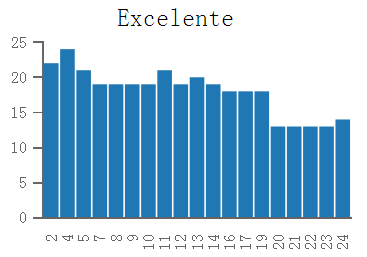
\includegraphics[scale=1.0]{figuras/loc.png}
		\caption{Qualidade da Métrica LOC nas \textit{Sprints} do Projeto SICG}
		\label{loc}
\end{figure}

\textbf{ACCM (Average Cyclomatic Complexity per Method)}

A Figura \ref{accm} mostra a qualidade da métrica ACCM. Esta métrica permanece com o intervalo de qualidade "Excelente" constante ao longo das \textit{sprints} do projeto.

\begin{figure}[H]
		\centering
			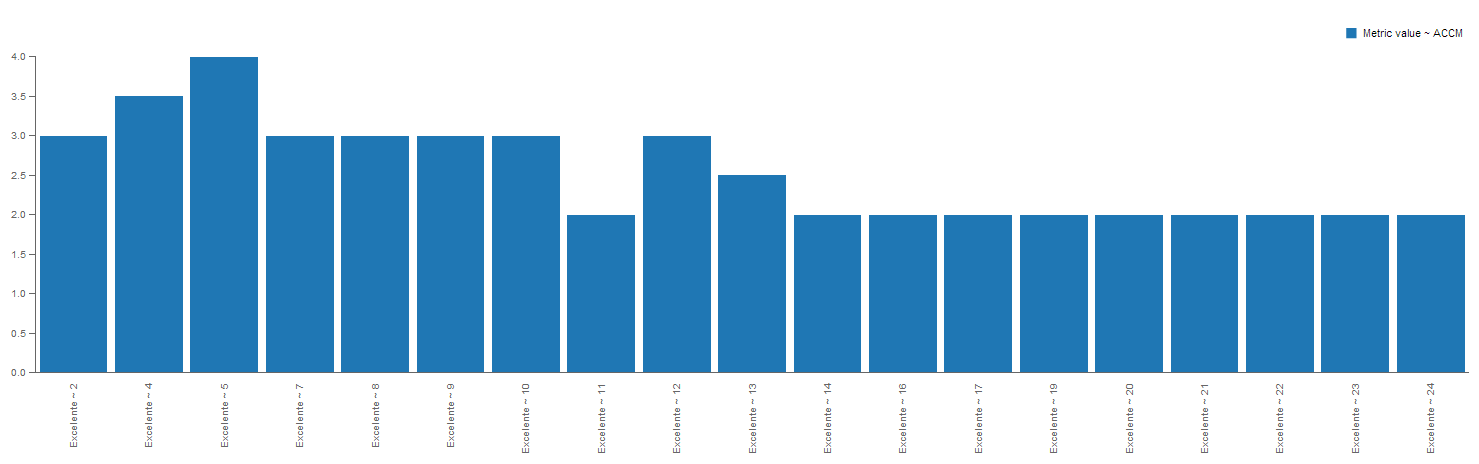
\includegraphics[scale=1.0]{figuras/accm.png}
		\caption{Qualidade da Métrica ACCM nas \textit{Sprints} do Projeto SICG}
		\label{accm}
\end{figure}

\textbf{AMLOC (Average Method Lines of Code)}

A Figura \ref{amloc} mostra a qualidade da métrica AMLOC. Esta métrica permanece com o intervalo de qualidade "Excelente" constante ao longo das \textit{sprints}do projeto.

\begin{figure}[H]
		\centering
			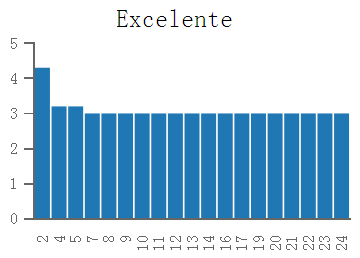
\includegraphics[scale=1.0]{figuras/amloc.png}
		\caption{Qualidade da Métrica AMLOC nas \textit{Sprints} do Projeto SICG}
		\label{amloc}
\end{figure}

\textbf{ACC (Afferent Connections per Class)}

A Figura \ref{acc} mostra a qualidade da métrica ACC. Esta métrica permanece com o intervalo de qualidade "Bom" constante ao longo das \textit{sprints} do projeto.

\begin{figure}[H]
		\centering
			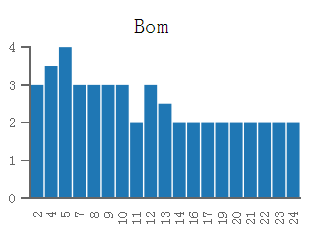
\includegraphics[scale=1.0]{figuras/acc.png}
		\caption{Qualidade da Métrica ACC nas \textit{Sprints} do Projeto SICG}
		\label{acc}
\end{figure}

\textbf{ANPM (Average Number of Parameters per Method)}

A Figura \ref{anpm} mostra a qualidade da métrica ANPM. Esta métrica permanece com o intervalo de qualidade "Excelente" constante ao longo das \textit{sprints} do projeto.

\begin{figure}[H]
		\centering
			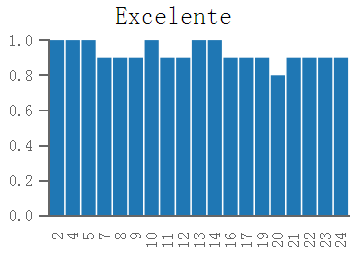
\includegraphics[scale=1.0]{figuras/anpm.png}
		\caption{Qualidade da Métrica ANPM nas \textit{Sprints} do Projeto SICG}
		\label{anpm}
\end{figure}

\textbf{CBO (Coupling Between Objects)}

A Figura \ref{cbo} mostra a qualidade da métrica CBO. Esta métrica permanece com o intervalo de qualidade "Ruim" constante ao longo das \textit{sprints} do projeto.

\begin{figure}[H]
		\centering
			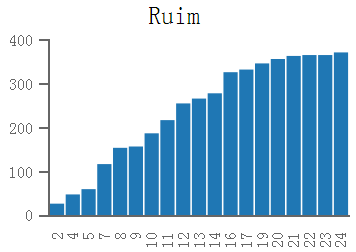
\includegraphics[scale=1.0]{figuras/cbo.png}
		\caption{Qualidade da Métrica CBO nas \textit{Sprints} do Projeto SICG}
		\label{cbo}
\end{figure}

\textbf{DIT(Depth of Inheritance Tree)}

A Figura \ref{dit} mostra a qualidade da métrica DIT. Esta métrica permanece com o intervalo de qualidade "Excelente" constante ao longo das \textit{sprints} do projeto.

\begin{figure}[H]
		\centering
			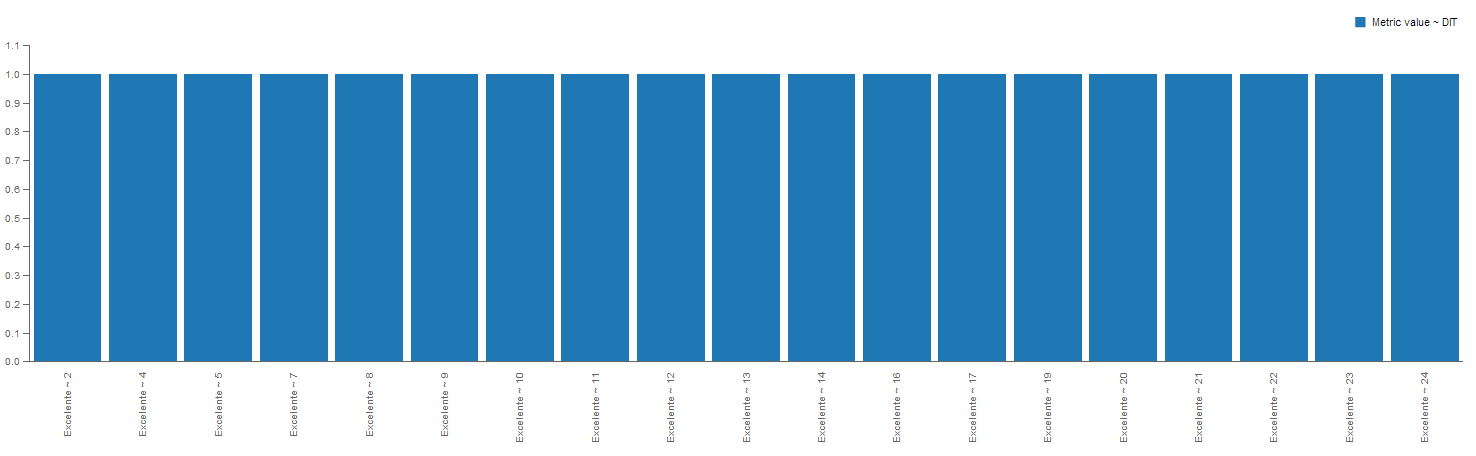
\includegraphics[scale=1.0]{figuras/dit.png}
		\caption{Qualidade da Métrica DIT nas \textit{Sprints} do Projeto SICG}
		\label{dit}
\end{figure}


\textbf{LCOM4 (Lack of Cohesion in Methods)} 

A Figura \ref{lcom4} mostra a qualidade da métrica LCOM4. Esta métrica inicia com o intervalo de qualidade "Bom" na primeira \textit{sprint} com entrega de \textit{software} (Sprint 2) e, posteriormente, permanece com o intervalo de qualidade "Regular" constante ao longo das demais \textit{sprints} do projeto.

\begin{figure}[H]
		\centering
			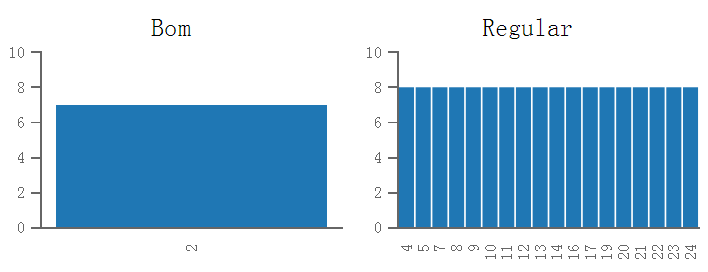
\includegraphics[scale=0.9]{figuras/lcom4.png}
		\caption{Qualidade da Métrica LCOM4  nas \textit{Sprints} do Projeto SICG}
		\label{lcom4}
\end{figure}

\textbf{NOC (Number of Children)}

A Figura \ref{noc} mostra a qualidade da métrica NOC. Esta métrica permanece com o intervalo de qualidade "Bom" constante ao longo das \textit{sprints} do projeto.

\begin{figure}[H]
		\centering
			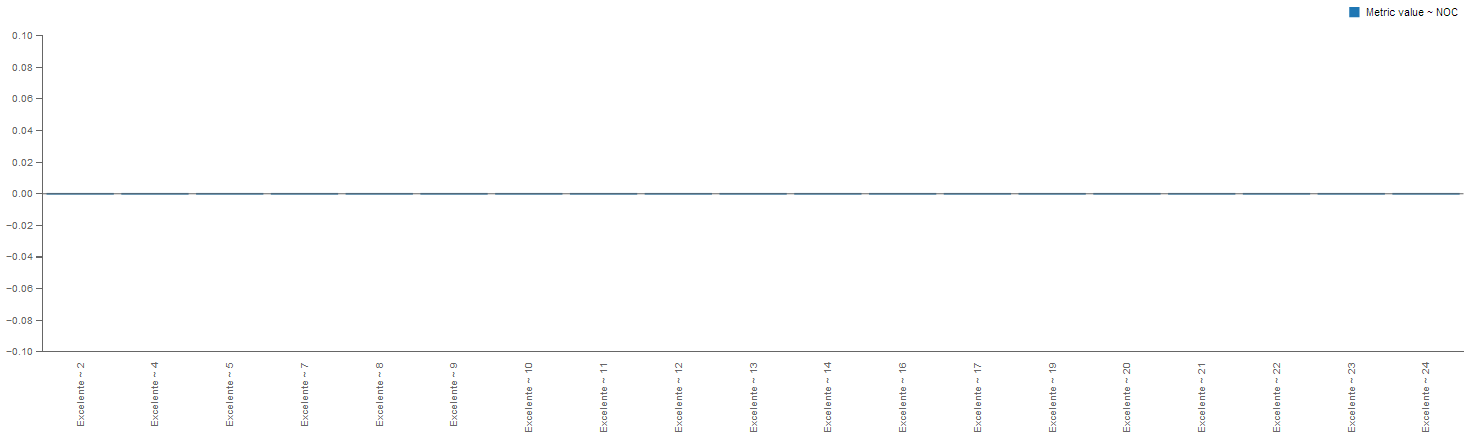
\includegraphics[scale=1.0]{figuras/noc.png}
		\caption{Qualidade da Métrica NOC nas \textit{Sprints} do Projeto SICG}
		\label{noc}
\end{figure}


\textbf{NOM (Number of Methods)} 

A Figura \ref{nom} mostra a qualidade da métrica NOM. Esta métrica permanece com o intervalo de qualidade "Bom" até a \textit{Sprint} 11 do projeto, a partir da \textit{Sprint} 12 o código fonte obtém uma melhoria e a métrica NOM passa a ter o intervalo de qualidade "Excelente" até a última \textit{sprint} analisada do projeto.

\begin{figure}[H]
		\centering
			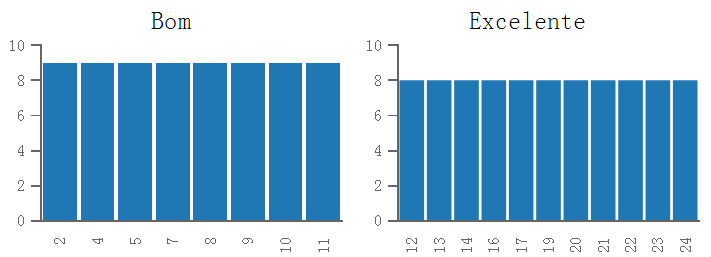
\includegraphics[scale=0.9]{figuras/nom.png}
		\caption{Qualidade da Métrica NOM nas \textit{Sprints} do Projeto SICG}
		\label{nom}
\end{figure}

\textbf{NPA (Number of Public Attributes)} 

A Figura \ref{npa} mostra a qualidade da métrica NPA. Esta métrica permanece com o intervalo de qualidade "Excelente" constante ao longo das \textit{sprints} do projeto.

\begin{figure}[H]
		\centering
			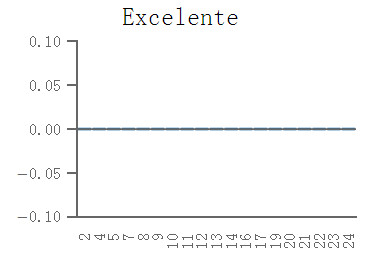
\includegraphics[scale=1.0]{figuras/npa.png}
		\caption{Qualidade da Métrica NPA nas \textit{Sprints} do Projeto SICG}
		\label{npa}
\end{figure}

\textbf{RFC (Response For a Class)} 

A Figura \ref{rfc} mostra a qualidade da métrica RFC. Esta métrica permanece com o intervalo de qualidade "Bom" constante ao longo das \textit{sprints} do projeto.

\begin{figure}[H]
		\centering
			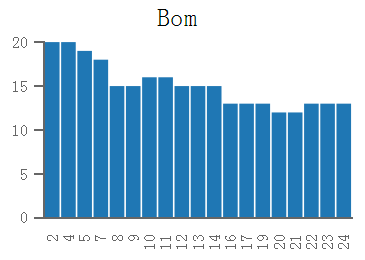
\includegraphics[scale=1.0]{figuras/rfc.png}
		\caption{Qualidade da Métrica RFC nas \textit{Sprints} do Projeto SICG}
		\label{rfc}
\end{figure}

A \textit{Sprint} 24 é a última \textit{sprint} do projeto e, portanto, é nela que foi entregue o código fonte final. Conforme a Fig. \ref{pizzatotal}, na análise da qualidade do código fonte dessa \textit{sprint}, observamos uma predominância do intervalo de qualidade "Excelente", o qual acontece em 7 métricas. O intervalo de qualidade "Bom" acontece em 3 métricas. O intervalo de qualidade "Regular" acontece em 1 métrica. E o intervalo de qualidade "Ruim" acontece em 1 métrica.

\begin{figure}[H]
		\centering
			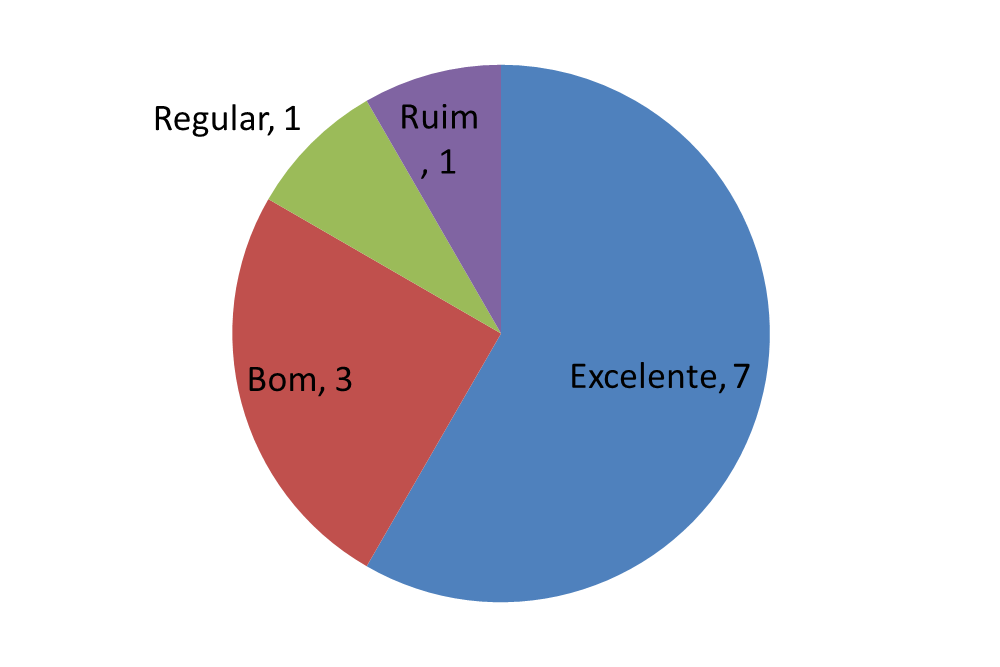
\includegraphics[scale=1.0]{figuras/pizzatotal.png}
		\caption{Qualidade Geral do Código Fonte}
		\label{pizzatotal}
\end{figure}


É possível perceber claramente que o resultado da métrica CBO desvirtua do resultado das demais métricas. Como mostrado na Tab. (\ref{intervalos}), para que a métrica CBO seja rotulada como "Ruim" o valor dela deve está acima de 9. Observando o gráfico da Fig. \ref{cbo}, vemos que na última \textit{sprint} do projeto esta métrica está próxima do valor 400.

A Figura \ref{percepcaoqualidade} mostra a percepção da qualidade do código fonte do SICG segundo os envolvidos no projeto (Scrum Master, Product Owner, Gestor do Contrato, Coordenador do Projeto, Fiscal Técnico e Desenvolvedores). Cerca de 66\% dos envolvidos consideraram  o intervalo de qualidade do código como "Excelente" e os demais consideraram
o intervalo de qualidade como "Bom".

\begin{figure}[H]
		\centering
			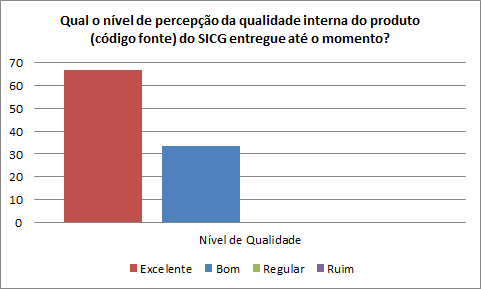
\includegraphics[scale=1.0]{figuras/percepcaoqualidade.png}
		\caption{Nível de Percepção da Qualidade do Código Fonte}
		\label{percepcaoqualidade}
\end{figure}

Assim, no que diz respeito a análise estática do código realizada, a qualidade interna do produto pode ser considerada satisfatória ao compararmos com o melhor \textit{software} livre encontrado na linguagem de programação Java, de acordo com os estudos de \citeonline{Meirelles2013}, sem considerarmos o impacto do resultado da métrica CBO. Além disso, há uma convergência com a também percepção satisfatória na dos envolvidos no projeto SICG, embora não tenhamos encontrado evidências de que o IPHAN realizava análise sistemática sobre tais métricas de qualidade de produto.

Ao analisarmos a qualidade interna do código fonte atribuindo um grande impacto do resultado da métrica CBO sobre a qualidade final (caso essa fosse a escolha do fiscal técnico do contrato), a qualidade do produto poderia ser considerada insatisfatória, e isso poderia contradizer a percepção dos usuários. Isso pode suscitar importantes discussões: i) o código pode estar altamente acoplado e possuir uma quantidade alta de oportunidades de refatoração no que diz respeito aos seguintes cenários: classes pouco coesa, interface dos métodos, classes com muitos filhos, classe com métodos grandes e/ou muitos condicionais, classe com muita exposição e complexidade estrutural ii) Essa alta medida pode estar sendo causada pelo uso de uma combinação de \textit{frameworks}; iii) a configuração de métricas escolhida pode não ser adequada para a comparação com a configuração de métricas analisadas; iv) a escala da medição pode não ter sido adequada. ; v) a eficiência e eficácia da aplicação das práticas ágeis relacionadas a qualidade interna do produto não foi atingida. De qualquer modo, carecemos de estudos mais aprofundados e controlados para investigar melhor a relação de causa e efeito entre as variáveis observadas e medidas.

No entanto, segundo \citeonline{Meirelles2013}, o uso de uma única métrica isolada na análise pode levar a interpretações errôneas tanto do lado do cliente quanto do lado do fornecedor. Com isso, essas métricas são reconhecidamente limitadas quando analisadas isoladamente. Assim, não é recomendado atribuir grande impacto do resultado do CBO na análise geral da qualidade interna do código fonte. O ideal é observar o comportamento de todas as métricas e extrair as informações necessárias para a melhoria da qualidade.

De acordo com as informações levantadas em entrevistas informais, o IPHAN disponibilizou o sistema desenvolvido para treinamento, por parte dos usuários, apenas na \textit{sprint} 21 e em ambiente de produção apenas ao final do projeto. Essa implantação tardia fere o valor do Manifesto Ágil de \textit{"Software operante..."} e poderia ter comprometido o funcionamento adequado final do sistema. Além disso, durante os ciclos do projeto, a vistoria técnica analisava se as classes estavam documentadas, como pedido no contrato, e se o modelo de dados era válido, o que evidencia a busca pela excelência da qualidade interna por parte dos gestores técnicos. Contudo, evidenciamos que a análise de qualidade do código fonte foi realizada apenas ao final do projeto por uma outra empresa contratada para aferir a qualidade, a RSI Informática Ltda. 


Os resultados das métricas analisadas nesse estudo que receberam rótulos de qualidade "Excelente" ou "Bom" se devem mais a aspectos considerados pela empresa contratada do que a capacidade própria do IPHAN em aferir e considerar os resultados da análise desta como conhecimento para, por exemplo, ser utilizado para o faturamento das OS's.

O fato de padrões de qualidade de métricas de código fonte não terem sido específicados no contrato e o fato de uma análise de qualidade de código de fonte não ter sido realizada durante os ciclos do projeto figuraram como risco ao projeto, uma vez que poderia ter comprometido o sucesso e a manutenibilidade do sistema.